\section{Entità e caratteristiche}
La realizzazione del secondo esercizio si caratterizza nell'estrazione di caratteristiche relativa ai calciatori professionisti della società sportiva italiana \textit{Internazionale Milano}. Per valutare l'efficacia delle espressioni utilizzate e provare la loro indipendenza dai ruoli dei calciatori, sono state provate per portieri, difensori, centrocampisti e attaccanti. Infatti alcuni siti collezionano statistiche differenti a seconda del ruolo del giocatore, inoltre ne associano strutture html differenti.

Si noti che tra le caratteristiche selezionate, ne sono state scelte alcune aggiuntive e specifiche per i vari siti trovati (e.g. il valore di mercato di un calciatore per il sito Transfermarket - vedi \ref{it:transfermarket}).

Le caratteristiche in questione sono le seguenti:
\begin{itemize}
\setlength\itemsep{0.1em}
    \item Nome e Cognome
    \item Data di nascita (o Eta)
    \item Posizione
    \item Piede
    \item Presenze
    \item Gol
    \item Assist
    \item Ammonizioni
    \item Espulsioni
\end{itemize}

\begin{table}[h]
    \centering
    \begin{tabular}{|c|c|c|}
        \hline
        \multicolumn{3}{|c|}{Caratteristiche aggiuntive}  \\
        \hline
        \textbf{Tranfermarket} & \textbf{Sito Inter} & \textbf{Sport Virgilio} \\
        \hline
        Valore di mercato & Altezza & Nazionale \\
        \hline
        & Contrasti vinti & Peso \\
        \hline
        & Disimpegni & Numero maglia \\
        \hline
        \multicolumn{3}{|c|}{}\\
        \hline
        \textbf{Tuttocalciatori} & \textbf{FootballDB} & \\
        \hline
        Scadenza di contratto & Squadra & \\
        \hline
        Procuratore & Minuti giocati & \\
        \hline
        Esordio in nazionale &  &\\
        \hline
    \end{tabular}
    \caption{Caratteristiche aggiuntive estratte dai relativi siti}
    \label{tab:my_label}
\end{table}
\newpage
Si noti che le statistiche sono relative all'anno corrente 2022/2023.
% \begin{itemize}
%     \item Transfermarket
%     \begin{itemize}
%         \item Valore di mercato
%     \end{itemize}
%     \item Sito Inter Ufficiale
%     \begin{itemize}
%         \item Altezza
%         \item Contrasti vinti
%         \item Disimpegni
%     \end{itemize}
%     \item Sport Virgilio
%     \begin{itemize}
%         \item Nazionale
%         % \item Nazionalità
%         \item Peso
%         \item Numero maglia
%         % \item Minuti giocati
%     \end{itemize}
%     \item Tuttocalciatori
%     \begin{itemize}
%         \item Scadenza contratto
%         \item Procuratore
%         \item Esordio in nazionale
%         % \item Presenze in nazionale
%         % \item Presenze nei campionati
%     \end{itemize}
%     \item Football Database
%     \begin{itemize}
%         \item Squadra
%         \item Minuti giocati
%     \end{itemize}
% \end{itemize}

\section{Siti web}
Per quanto riguardo i siti web, ne sono stati scelti 5 ed in ognuno individuate 5, o più, pagine web:
\begin{enumerate}
\setlength\itemsep{0.1em}
    \item \href{https://www.transfermarkt.it/inter-mailand/startseite/verein/46/saison_id/2022}{Transfermarket}\label{it:transfermarket}
    \begin{enumerate}
        \item \href{https://www.transfermarkt.it/alessandro-bastoni/profil/spieler/315853}{Alessandro Bastoni}
        \item \href{https://www.transfermarkt.it/lautaro-martinez/profil/spieler/406625}{Lautaro Martinez}
        \item \href{https://www.transfermarkt.it/edin-dzeko/profil/spieler/28396}{Edin Dzeko}
        \item \href{https://www.transfermarkt.it/henrikh-mkhitaryan/profil/spieler/55735}{Henrikh Mkhitaryan}
        \item  \href{https://www.transfermarkt.it/nicolo-barella/profil/spieler/255942}{Nicolo Barella}
        \item \href{https://www.transfermarkt.it/samir-handanovic/profil/spieler/28021}{Samir Handanovic}
    \end{enumerate}
    \item \href{https://www.inter.it/it/teams/prima-squadra?role=tutti}{Sito Inter Ufficiale}
    \begin{enumerate}
        \item \href{https://www.inter.it/it/squadra/prima-squadra/stefan-de-vrij}{Stefan de Vrij}
        \item \href{https://www.inter.it/it/squadra/prima-squadra/raoul-bellanova}{Raoul Bellanova}
        \item \href{https://www.inter.it/it/squadra/prima-squadra/francesco-acerbi}{Francesco Acerbi}
        \item \href{https://www.inter.it/it/squadra/prima-squadra/dimarco}{Di Marco}
        \item  \href{https://www.inter.it/it/squadra/prima-squadra/milan-skriniar}{Milan Skriniar}
        \item \href{https://www.inter.it/it/squadra/prima-squadra/hakan-calhanoglu}{Hakan Calhanoglu}
        \item \href{https://www.inter.it/it/squadra/prima-squadra/lautaro-martinez}{Lautaro Martinez}
        \item \href{https://www.inter.it/it/squadra/prima-squadra/andre-onana}{Andre Onana}
    \end{enumerate}
    \item \href{https://sport.virgilio.it/calcio/giocatori/}{Sport Virgilio}\label{it:prod3}
    \begin{enumerate}
        \item \href{https://sport.virgilio.it/calcio/giocatori/robin_gosens/}{Robin Gosens}
        \item \href{https://sport.virgilio.it/calcio/giocatori/marcelo_brozovic/}{Marcelo Brozovic}
        \item \href{https://sport.virgilio.it/calcio/giocatori/matteo_darmian/}{Matteo Darmian}
        \item \href{https://sport.virgilio.it/calcio/giocatori/joaquin_correa/}{Joaquin Correa}
        \item \href{https://sport.virgilio.it/calcio/giocatori/romelu_lukaku/}{Romelu Lukaku}
        \item \href{https://sport.virgilio.it/calcio/giocatori/samir_handanovic/}{Samir Handanovic}
        \item \href{https://sport.virgilio.it/calcio/giocatori/johan_vasquez/}{Johan Vasquez}
    \end{enumerate}
    \item \href{https://www.tuttocalciatori.net/rosa/f.c.-internazionale}{Tuttocalciatori}
    \begin{enumerate}
        \item \href{https://www.tuttocalciatori.net/Onana_Andr%E8}{Andre Onana}
        \item \href{https://www.tuttocalciatori.net/Handanovic_Samir}{Samir Handanovic}
        \item \href{https://www.tuttocalciatori.net/Cordaz_Alex}{Alex Cordaz}
        \item \href{https://www.tuttocalciatori.net/?mod=cc1&par=5646}{Danilo d'Ambrosio}
        \item \href{https://www.tuttocalciatori.net/Asllani_Kristjan}{Kristjan Asllani}
        \item \href{https://www.tuttocalciatori.net/Dzeko_Edin}{Edin Dzeko}
        \item \href{https://www.tuttocalciatori.net/Dybala_Paulo}{Paulo Dybala}
    \end{enumerate}
    \item \href{https://www.footballdatabase.eu/en/club/team/16-inter_milan/2022-2023}{Football Database}
    \begin{enumerate}
        \item \href{https://www.footballdatabase.eu/en/player/details/279784-lautaro-martinez}{Lautaro Martinez}
        \item \href{https://www.footballdatabase.eu/en/player/details/70663-romelu-lukaku}{Romelu Lukaku}
        \item \href{https://www.footballdatabase.eu/en/player/details/252538-nicolo-barella}{Nicolo Barella}
        \item \href{https://www.footballdatabase.eu/en/player/details/112559-marcelo-brozovic}{Marcelo Brozovic}
        \item \href{https://www.footballdatabase.eu/en/player/details/223558-robin-gosens}{Robin Gosens}
        \item \href{https://www.footballdatabase.eu/en/player/details/110489-francesco-acerbi}{Francesco Acerbi}
        \item \href{https://www.footballdatabase.eu/en/player/details/244843-andre-onana}{Andre Onana}
        \item \href{https://www.footballdatabase.eu/en/player/details/11916-samir-handanovic}{Samir Handanovic}
        \item \href{https://www.footballdatabase.eu/en/player/details/244461-gianluca-mancini}{Gianluca Mancini}
    \end{enumerate}
\end{enumerate}

\section{Analisi strutturale delle pagine web}
L'analisi strutturale, così come per il primo esercizio, è stata necessaria per comprendere in che modo agire per trovare le espressioni più adatte per l'obiettivo. In particolare, questo passo è stato ripetuto per ogni sito (e quindi ogni sua pagina web), poiché ognuno di essi risulta avere un struttura ovviamente diversa.

\section{Web scraping}
L'approccio per il web scraping, comune con quello adottato per il primo esercizio, si è basato su due principali tipologie di espressioni: la prima prevede l'individuazione di tag caratterizzati da un \texttt{id} univoco, oppure da determinati valori presenti nell'attributo \texttt{class}, mentre la seconda si basa sul testo presente in un tag vicino al dato d'interese, per cui, trovato questo punto di partenza, si visita il DOM per trovare l'informazione localizzata nelle vicinanze.

Si noti che la prima caratteristica ricercata è il nome e cognome dei calciatori, sebbene in alcune pagine si posiziona in un unico tag, in altre si localizzano in tag separati e vicini fra loro nel DOM. Quindi in quest'ultime pagine è stata utilizzata una metodologia per cui nome e cognome sono stati separatamente individuati e messi in pipe, in questo modo entrambi i risultati sono stati stampati (questi approcci sono visbili in \ref{se:transfermarket} e \ref{se:fdb}). 

Per quanto riguarda le altre caratteristiche, è possibile che alcuni siti non le memorizzino o che le collezionino solo per certi ruoli. Questo comportamento giustifica quelle espressioni che riportano array vuoti come risultato, per cui non è stato possibile raccogliere tutte le caratteristiche in tutte le pagine dei siti.

\newpage
\subsection{Transfermarket}\label{se:transfermarket}
Il problema sorto per questo sito è relativo al nome e cognome dei calciatori. Infatti, come accennato in precedenza, per questo sito (e le relative pagine) il nome ed il cognome, presenti in tag differenti, sono stati estratti con due espressioni \textit{XPath} separate, ma poi messe in pipe.
\begin{table}[h!]
    \centering
    \begin{tabular}{|l|>{\color{xpath}}l|}
    \hline
        \textbf{Nome e Cognome} & \thead{\$x("//header[contains\\(@itemtype,'https://schema.org/Person')]\\/div/h1/span/following-sibling::text()[1] |\\ //header[contains\\(@itemtype,'https://schema.org/Person')]\\/div/h1/span/following-sibling::strong/text()")} \\
    \hline
        \textbf{Data di nascita} & \thead{\$x("(//span[text()='Data di nascita:']\\/following-sibling::span)[1]/a/text()")}\\
    \hline
        \textbf{Posizione} & \thead{\$x("(//span[text()='Posizione:']\\/following-sibling::span)[1]/text()")}\\
    \hline
        \textbf{Piede} & \thead{\$x("(//span[text()='Piede:']\\/following-sibling::span)[1]/text()")}\\
    \hline
        \textbf{Presenze} & \thead{\$x("//span[text()='Partite']/parent::div\\/following-sibling::a/text()")} \\
    \hline
        \textbf{Gol} & \thead{\$x("//span[text()='Reti']/parent::div\\/following-sibling::a/text()")}\\
    \hline
        \textbf{Assist} & \thead{\$x("//span[text()='Assist']/parent::div\\/following-sibling::a/text()")}\\
    \hline
        \textbf{Ammonizioni} & \thead{\$x("//span[text()='Ammonizioni']/parent::div\\/following-sibling::a/text()")}\\
    \hline
        \textbf{Espulsioni} & \thead{\$x("//span[text()='Espulsioni']/parent::div\\/following-sibling::a/text()")}\\
    \hline
    \multicolumn{2}{|c|}{Caratteristiche aggiuntive} \\
    \hline
        \textbf{Valore di mercato} & \thead{\$x("//div[text()='Valore attuale:']\\/following-sibling::div/a/text()")}\\
    \hline
    \end{tabular}
    \caption{Caratteristiche ed espressioni per Transfermarket}
    \label{tab:my_label}
\end{table}
\begin{figure}
    \centering
    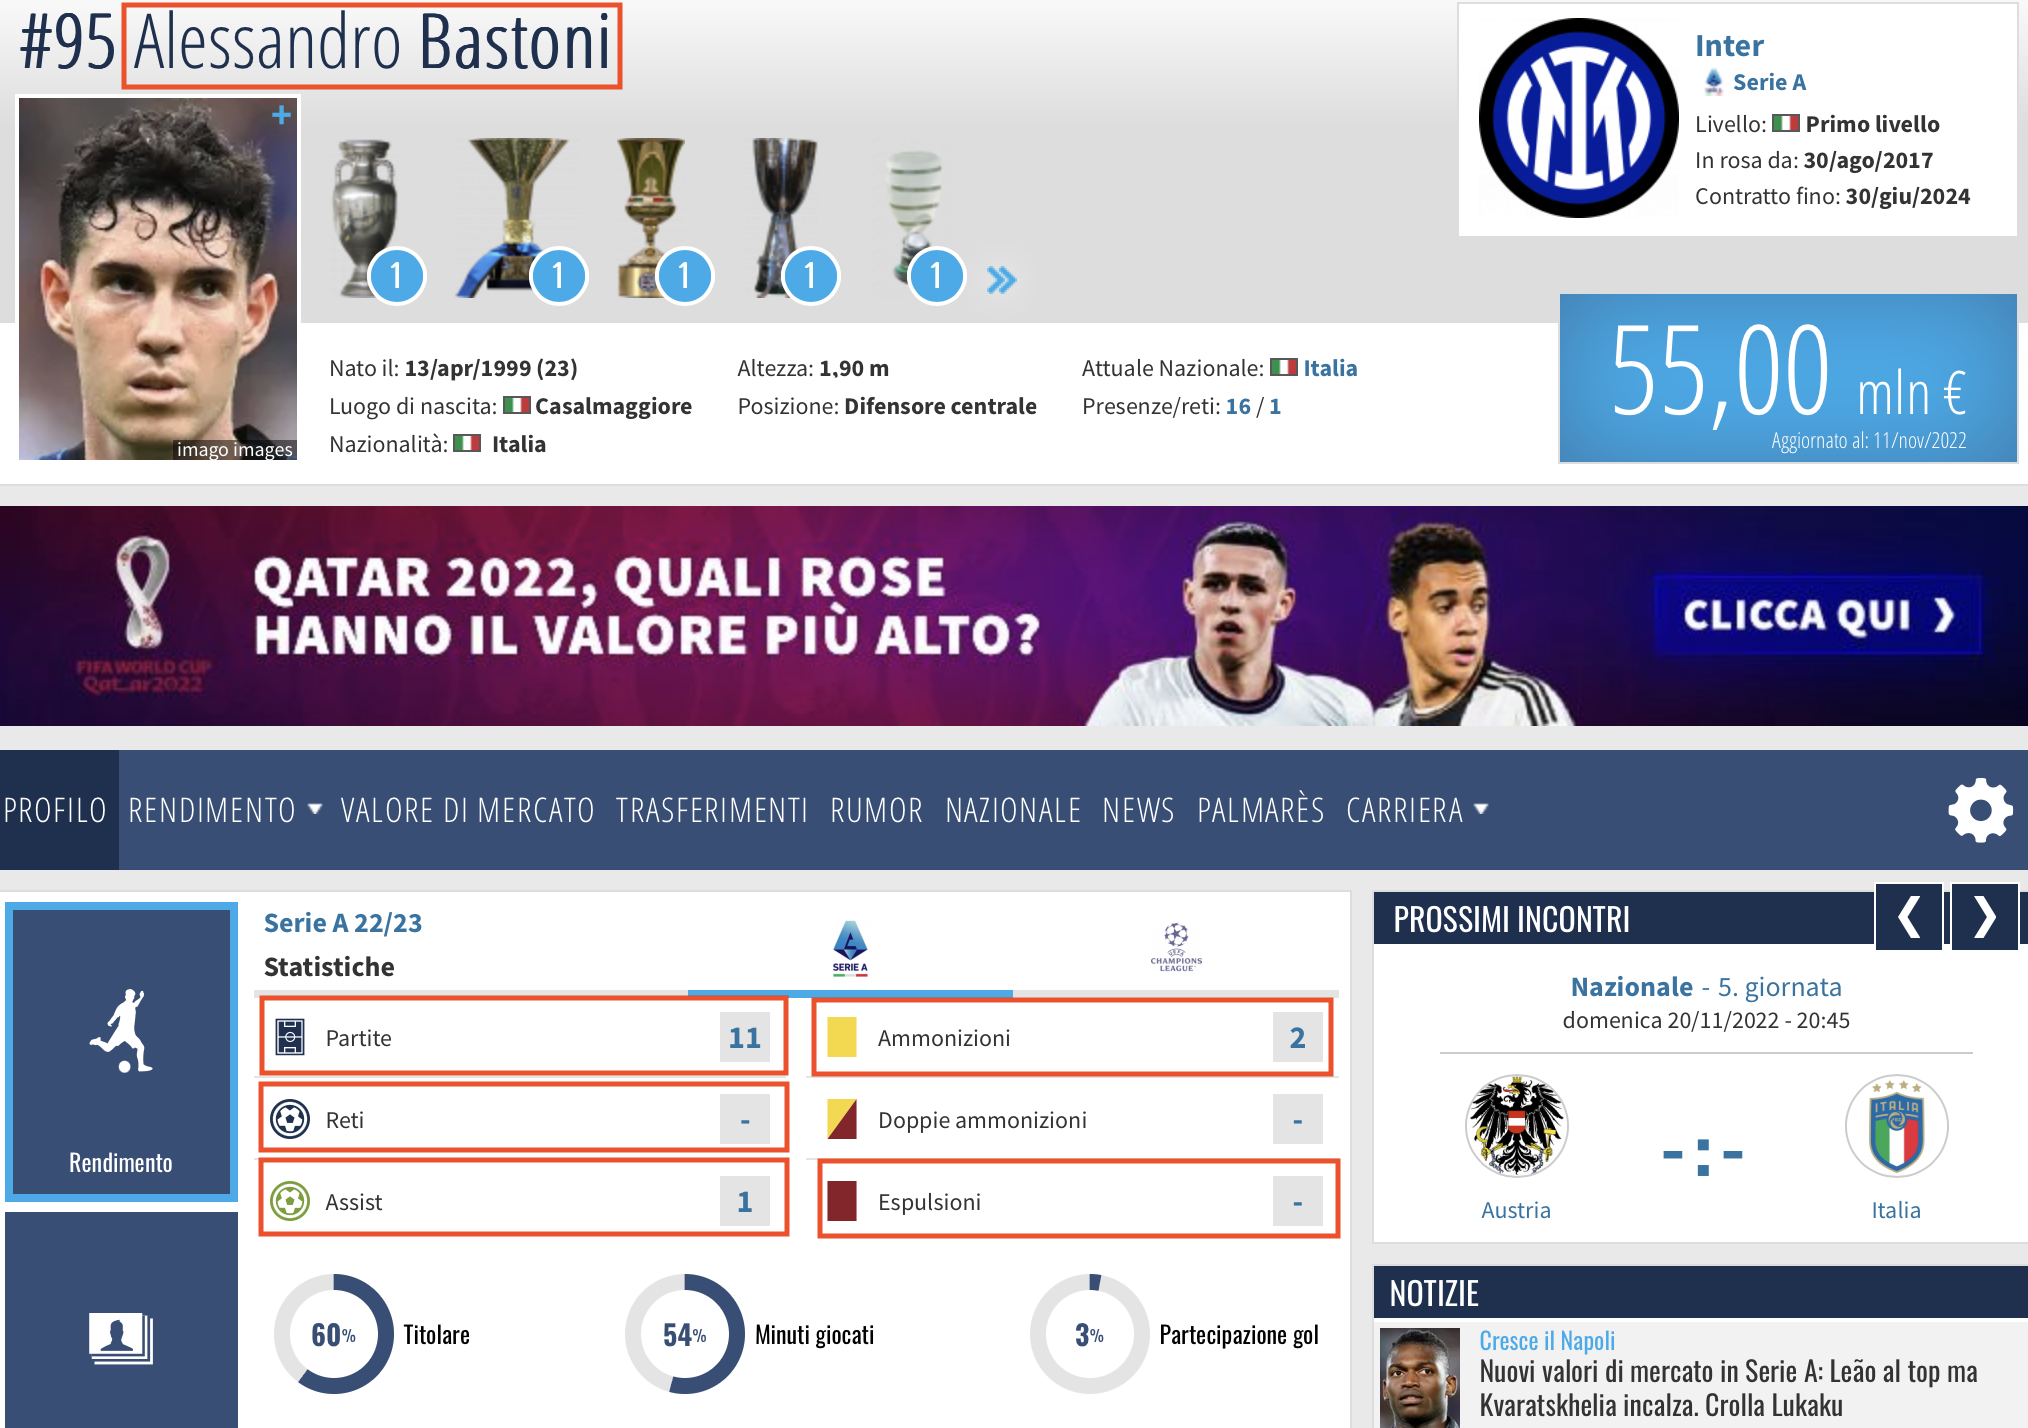
\includegraphics[scale=0.4]{img/Transfermarket1.png}
    \caption{Esempio di una pagina web di Transfermarket}
    \label{fig:Transfermarket1}
\end{figure}
\begin{figure}
    \centering
    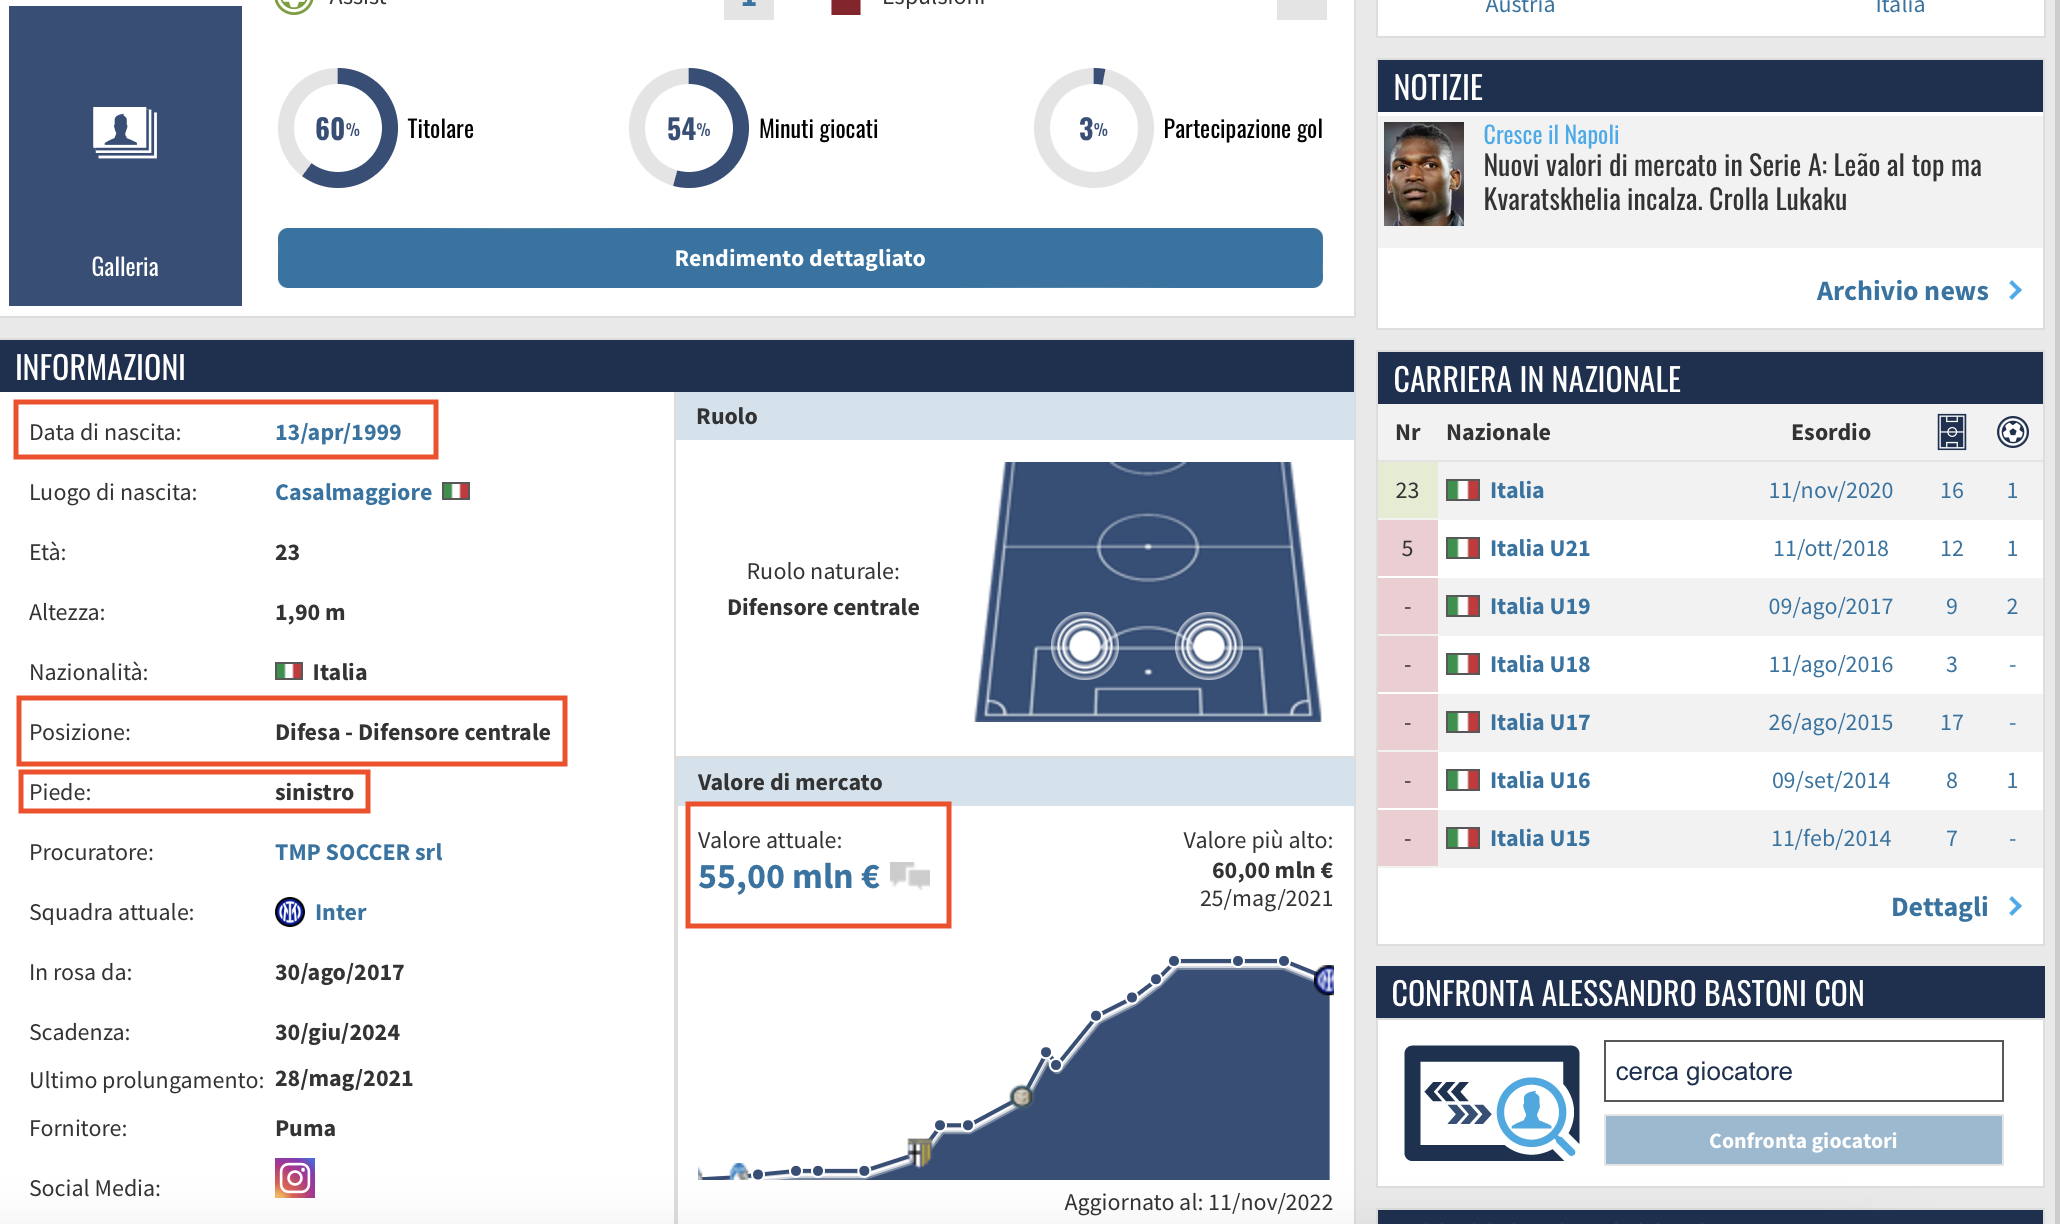
\includegraphics[scale=0.4]{img/Transfermarket2.png}
    \caption{Esempio di una pagina web di Transfermarket (continuo della pagina vista in \ref{fig:Transfermarket1})}
    \label{fig:Transfermarket2}
\end{figure}

\newpage
\subsection{Sito Inter Ufficiale}
\begin{table}[h!]
    \centering
    \begin{tabular}{|l|>{\color{xpath}}l|}
    \hline
        \textbf{Nome e Cognome} & \thead{\$x("//div[contains(@class,'css-1riajt')]\\/div[contains(@class,'css-79elbk')]\\/h1[contains(@class,'css-oq49di')]/span/text()")} \\
    \hline
        \textbf{Età} & \thead{\$x("//p[text()='Età']\\/preceding-sibling::p/text()")}\\
    \hline
        \textbf{Posizione} & \thead{\$x("//span[contains(@class,'css-jpejlw')]\\/text()")}\\
    \hline
        \textbf{Piede} & \thead{}\\
    \hline
        \textbf{Presenze} & \thead{\$x("//p[text()='Partite giocate']\\/following-sibling::p/span/text()")} \\
    \hline
        \textbf{Gol} & \thead{\$x("//p[text()='Gol segnati']\\/following-sibling::p/span/text()")}\\
    \hline
        \textbf{Assist} & \thead{}\\
    \hline
        \textbf{Ammonizioni} & \thead{\$x("//p[text()='Cartellini gialli']\\/following-sibling::p/span/text()")}\\
    \hline
        \textbf{Espulsioni} & \thead{\$x("//p[text()='Cartellini rossi']\\/following-sibling::p/span/text()")}\\
    \hline
    \multicolumn{2}{|c|}{Caratteristiche aggiuntive} \\
    \hline
        \textbf{Altezza} & \thead{\$x("(//p[text()='Altezza']\\/preceding-sibling::p/text())[1]")}\\
    \hline
        \textbf{Contrasti vinti} & \thead{\$x("//p[text()='Contrasti vinti']\\/following-sibling::p/span/text()")} \\
    \hline
        \textbf{Disimpegni} & \thead{\$x("//p[text()='Disimpegni']\\/following-sibling::p/span/text()")} \\
    \hline
    \end{tabular}
    \caption{Caratteristiche ed espressioni per il Sito Inter Ufficiale}
    \label{tab:my_label}
\end{table}
\begin{figure}
    \centering
    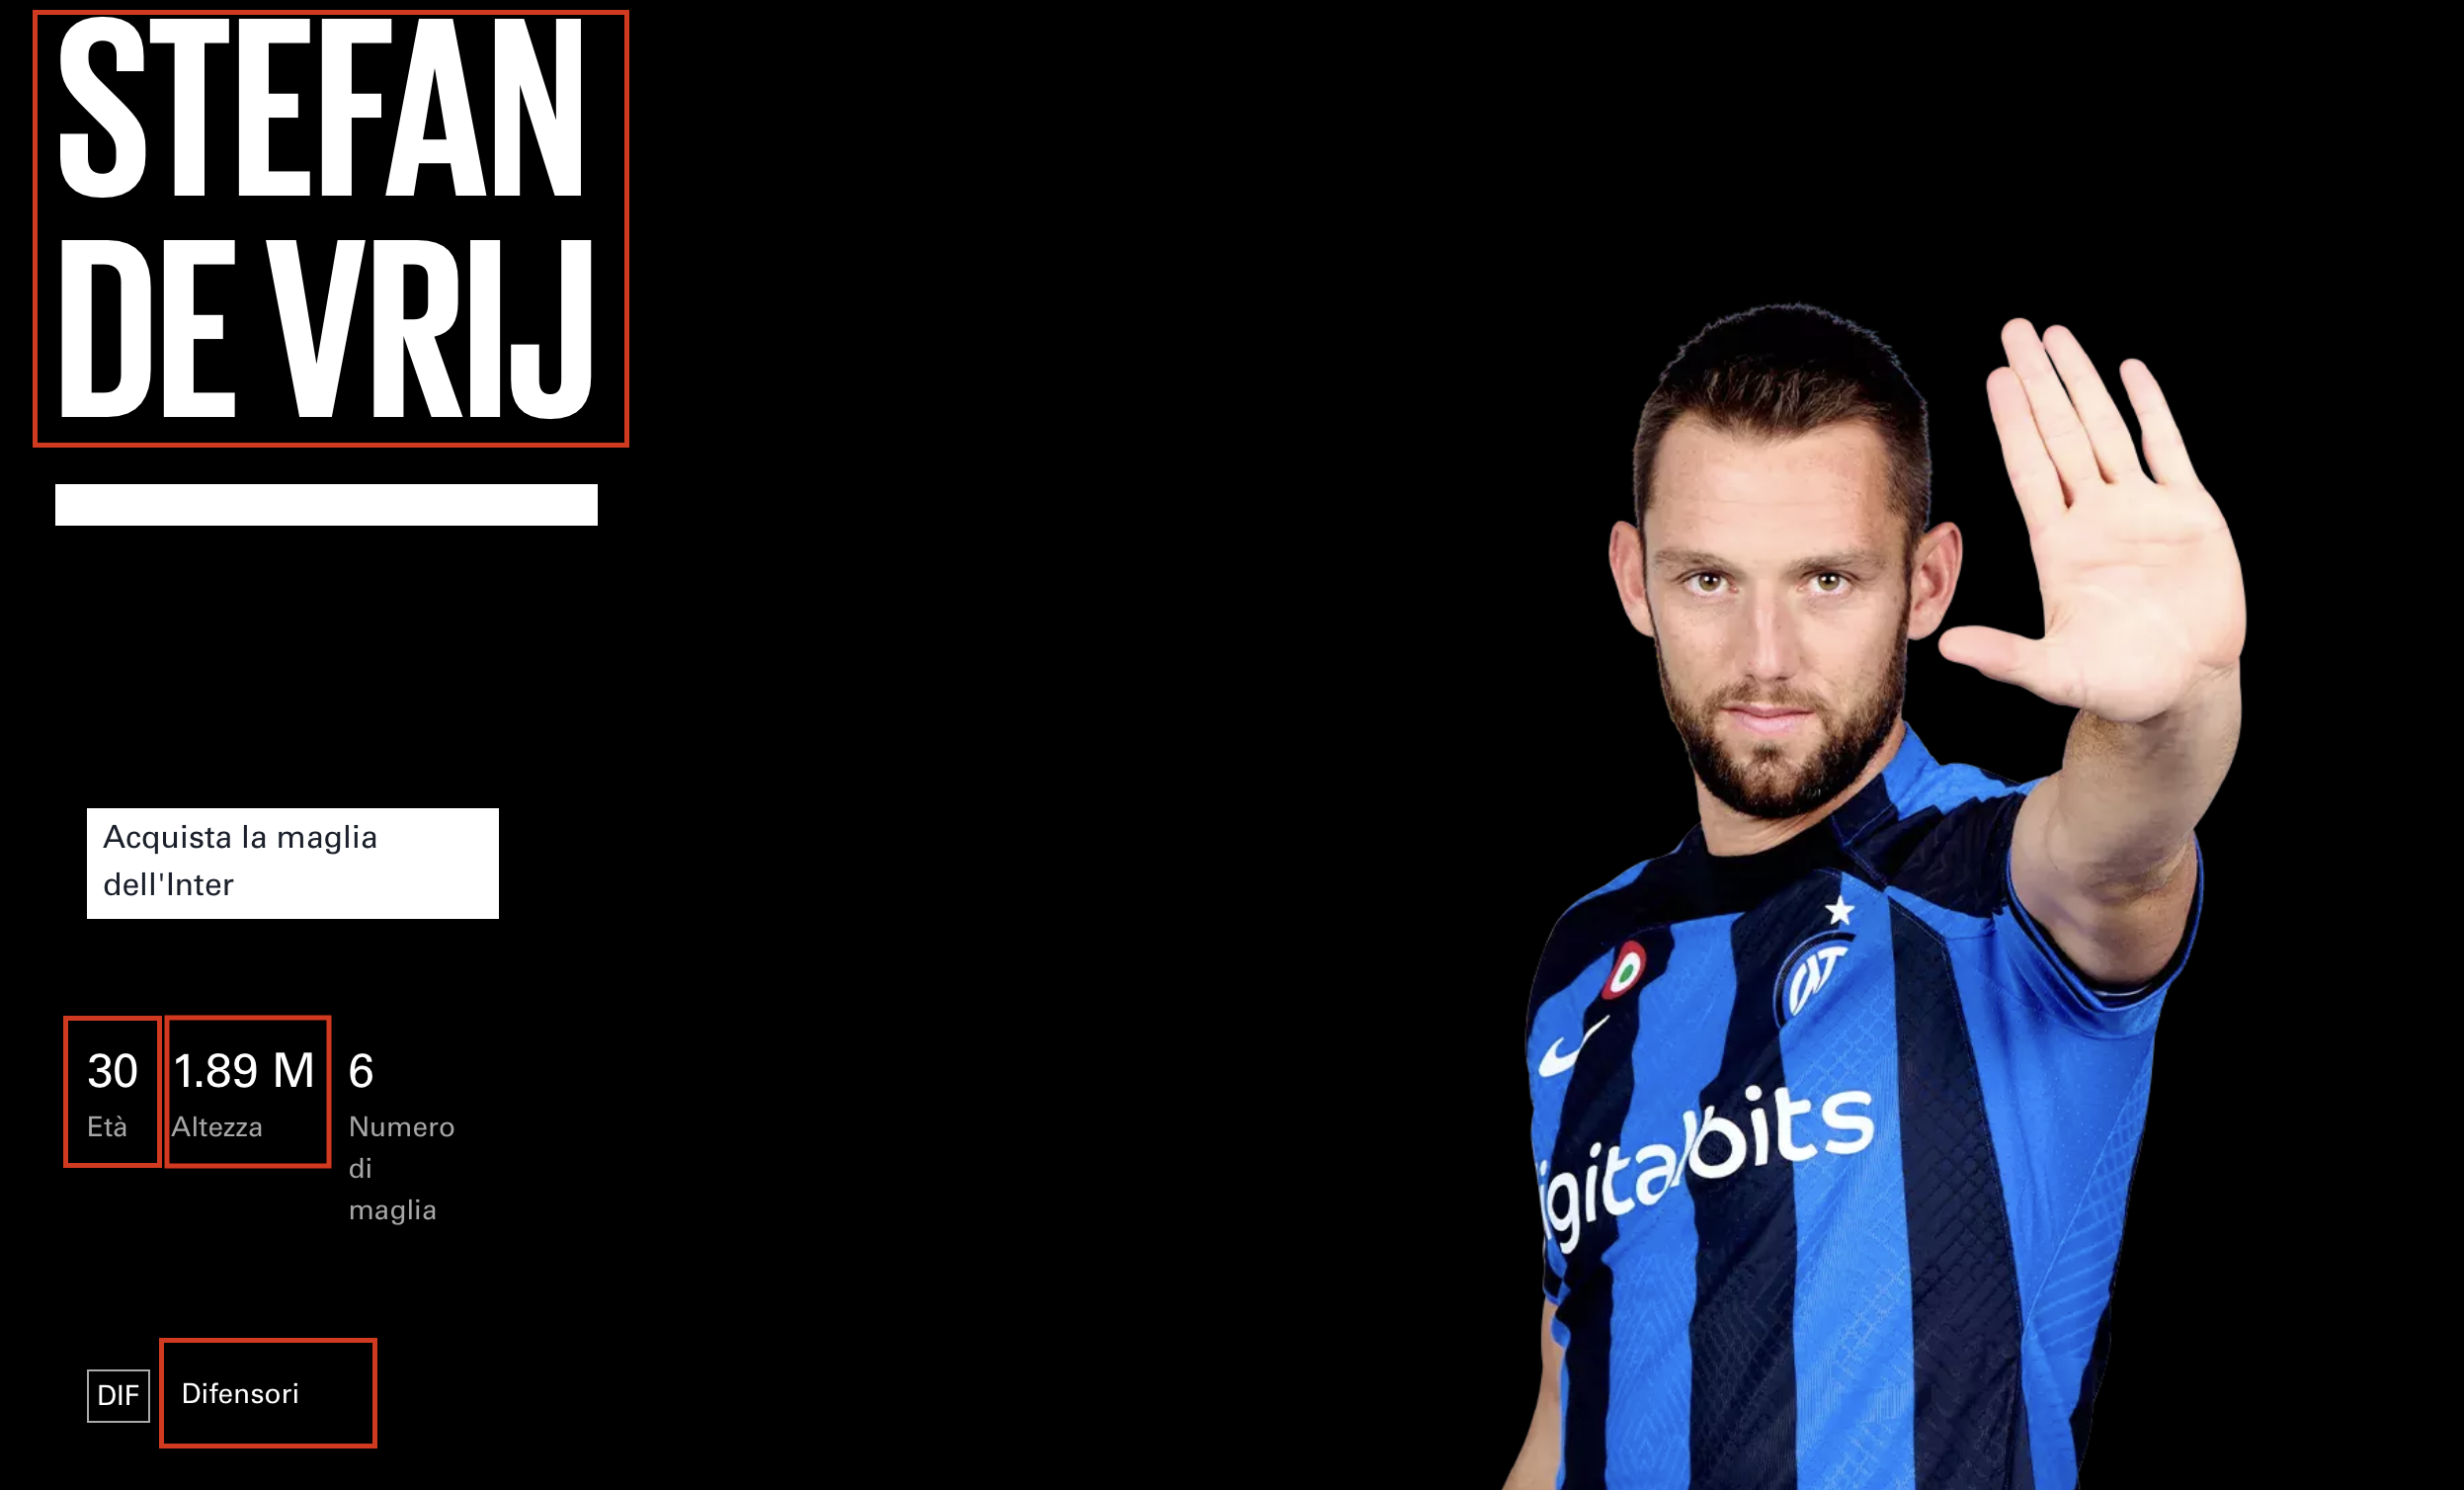
\includegraphics[scale=0.22]{img/inter1.png}
    \caption{Esempio pagina web per il Sito Inter Ufficiale (1)}
    \label{fig:inter1}
\end{figure}
\begin{figure}
    \centering
    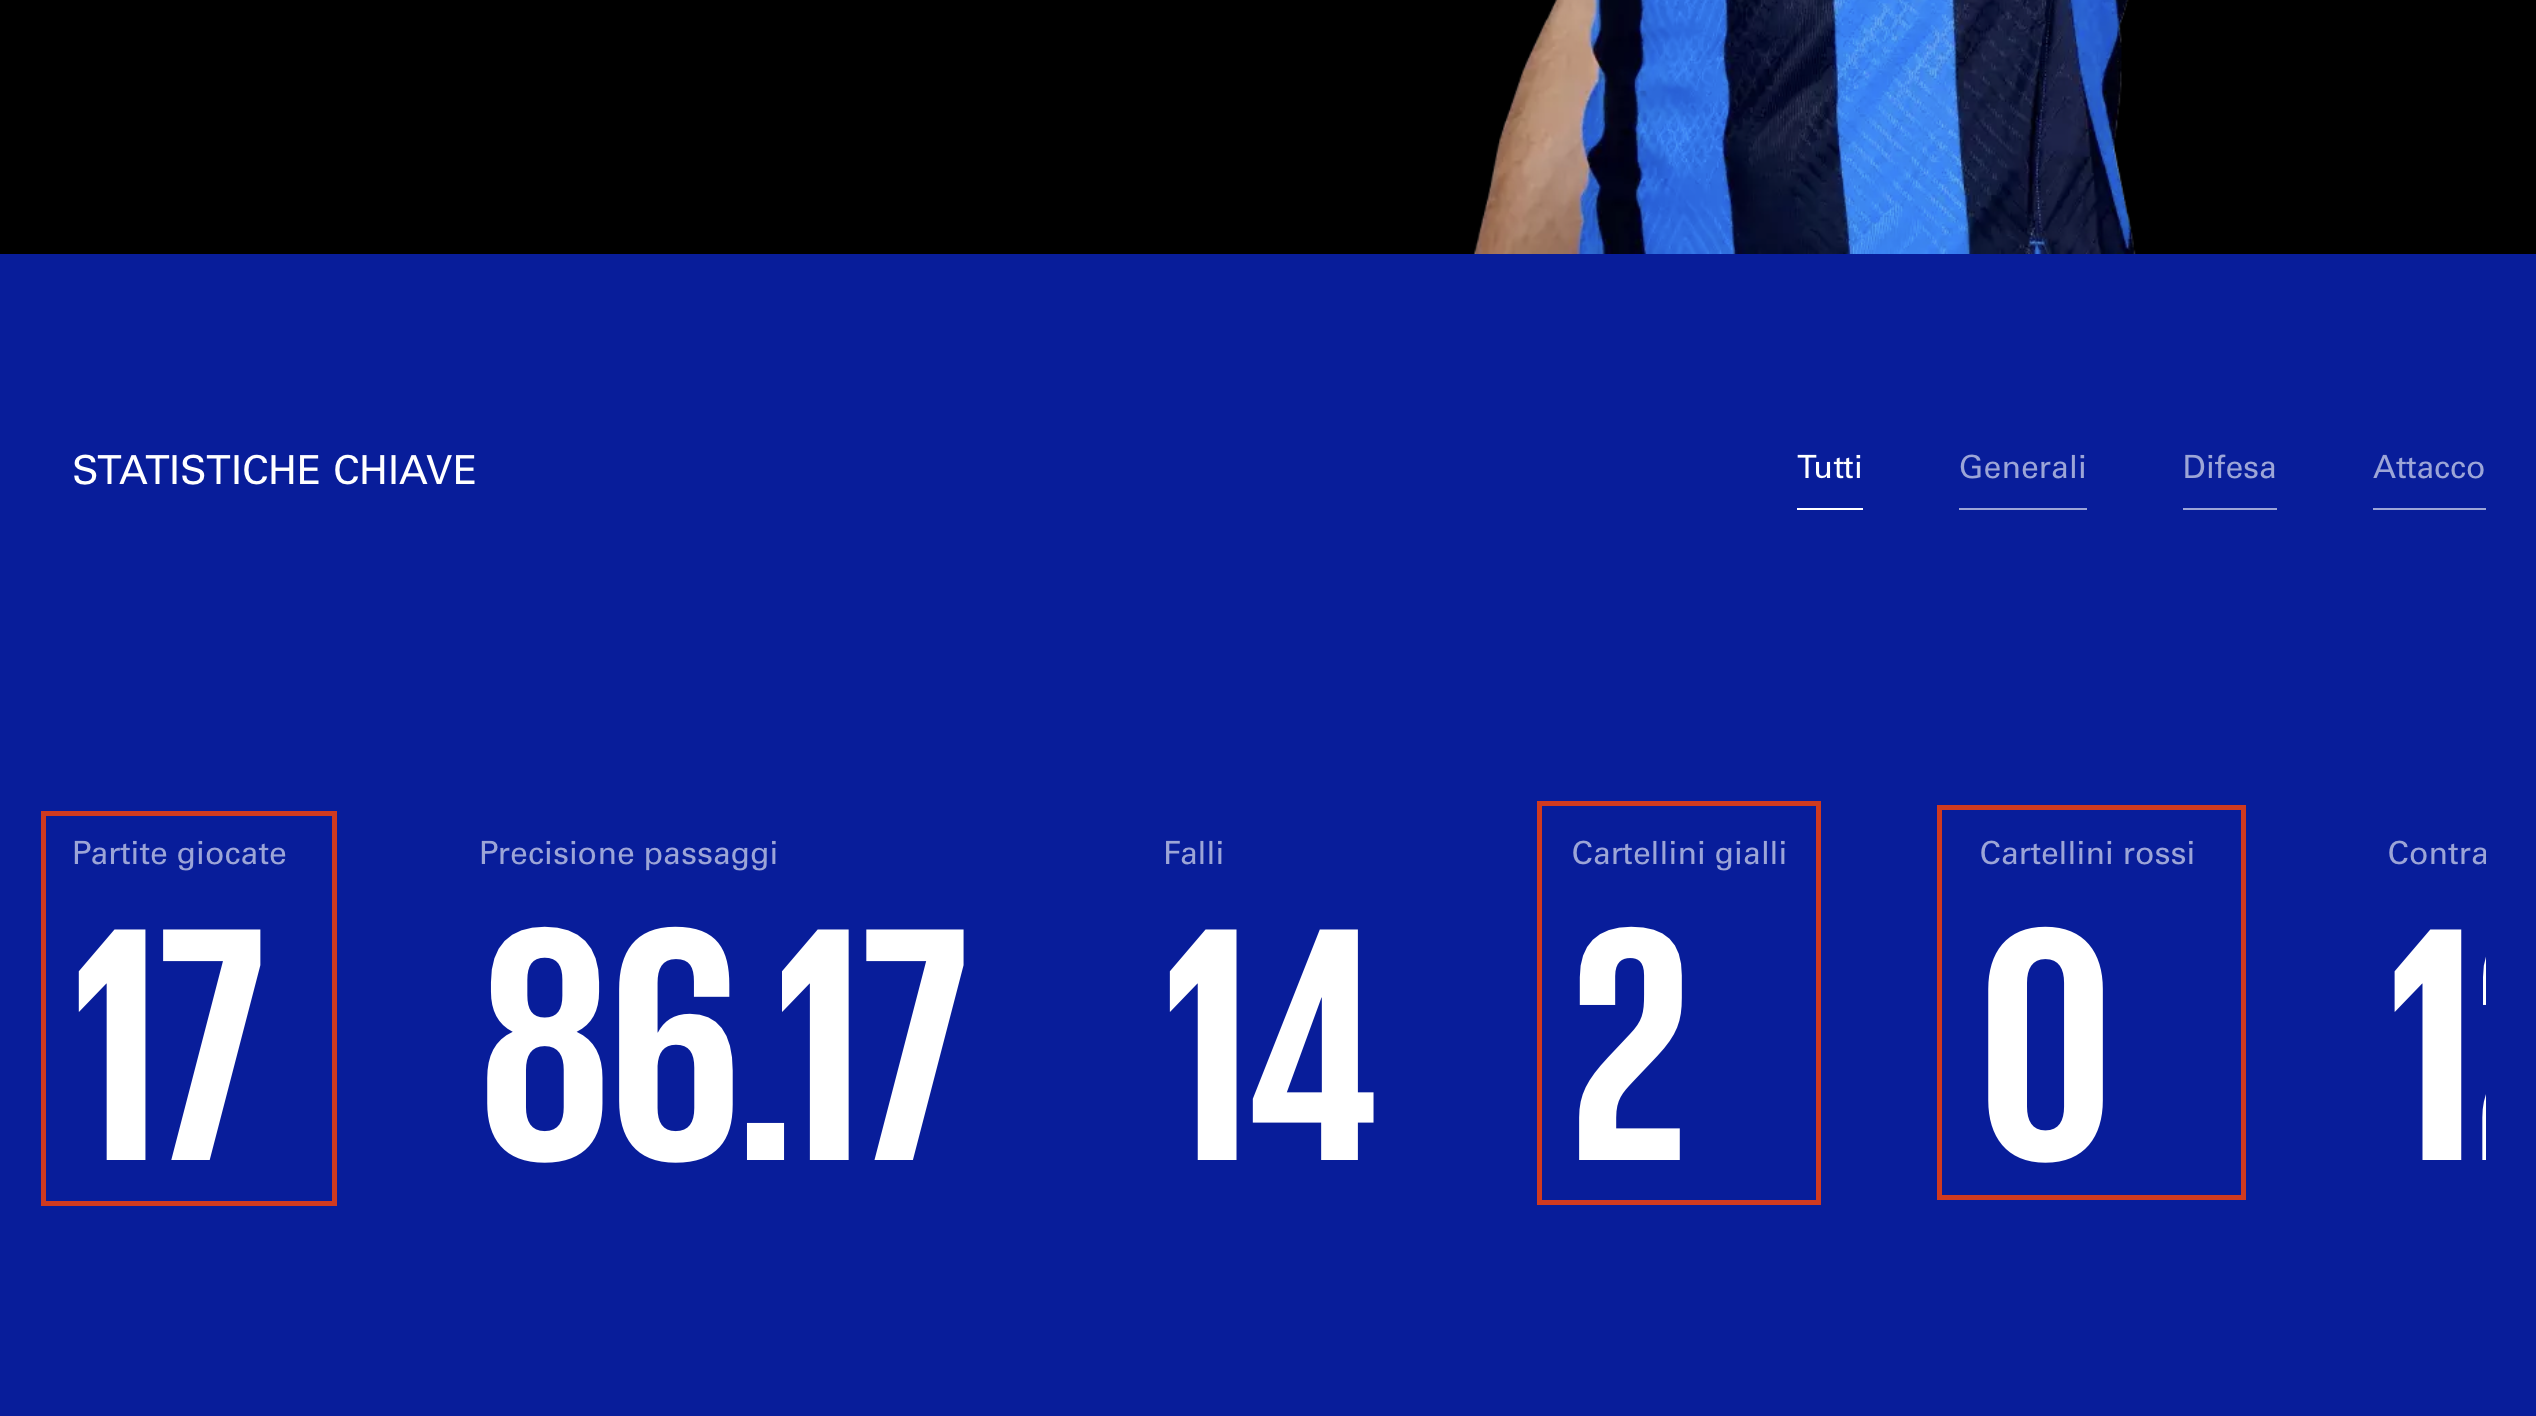
\includegraphics[scale=0.22]{img/inter2.png}
    \caption{Esempio pagina web per il Sito Inter Ufficiale (2)}
    \label{fig:inter1}
\end{figure}
\begin{figure}
    \centering
    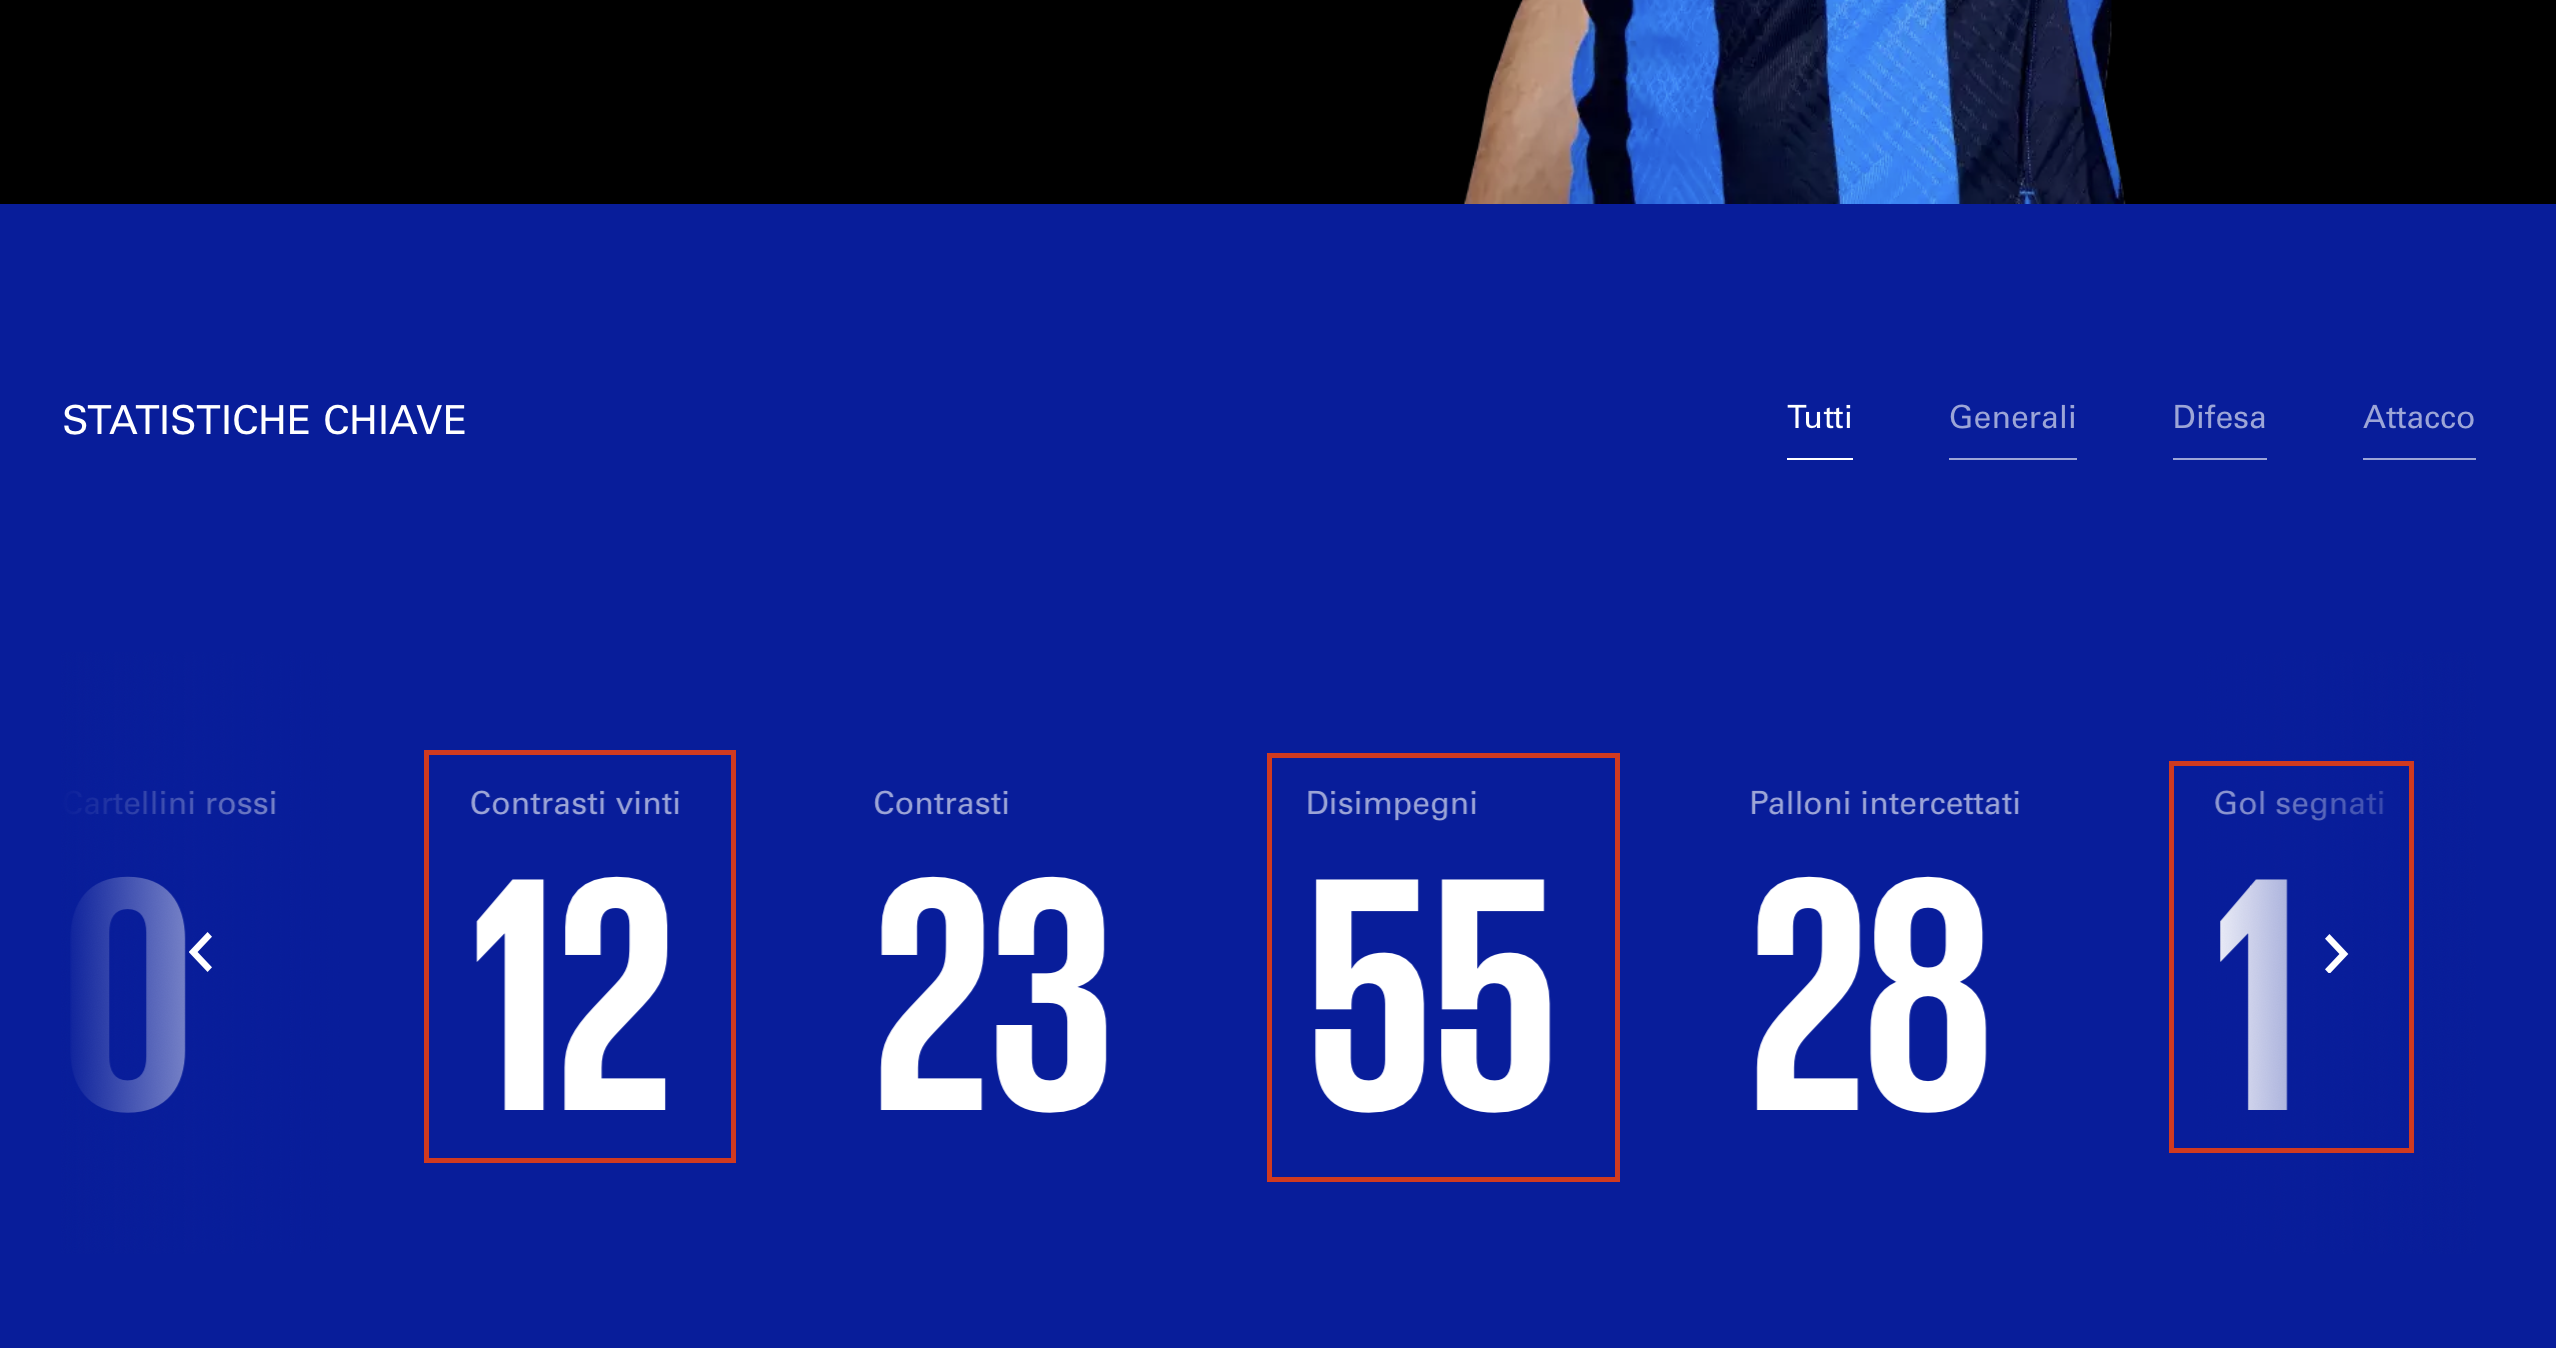
\includegraphics[scale=0.22]{img/inter3.png}
    \caption{Esempio pagina web per il Sito Inter Ufficiale (3)}
    \label{fig:inter1}
\end{figure}

\newpage
\subsection{Sport Virgilio}
In questo sito è stato osservato che per alcuni ruoli, come i portieri, alcune informazioni (i.e. gol e assist) non vengono mostrate.
\begin{table}[h!]
    \centering
    \begin{tabular}{|l|>{\color{xpath}}l|}
    \hline
        \textbf{Nome e Cognome} & \thead{\$x("//h1[contains(@class, 'title-page')]/text()")} \\
    \hline
        \textbf{Età} & \thead{\$x("//b[text()='Età:']\\/following-sibling::text()")}\\
    \hline
        \textbf{Posizione} & \thead{\$x("//*[contains(text(), 'Ruolo')]\\/following-sibling::text()")}\\
    \hline
        \textbf{Piede} & \thead{\$x("//b[text()='Piede preferito:']\\/following-sibling::text()")}\\
    \hline
        \textbf{Presenze} & \thead{\$x("//ul[@id='stats-leagues']\\//*[contains(text(),'Partite disputate')]\\/preceding-sibling::*/text()")} \\
    \hline
        \textbf{Gol} & \thead{\$x("(//span[text()='Gol fatti']\\/preceding-sibling::span/text())[1]")}\\
    \hline
        \textbf{Assist} & \thead{\$x("(//span[text()='Assist']\\/preceding-sibling::span/text())[1]")}\\
    \hline
        \textbf{Ammonizioni} & \thead{\$x("//ul[@id='stats-leagues']\\//*[contains(text(),'Cartellini gialli')]\\/preceding-sibling::*/text()")}\\
    \hline
        \textbf{Espulsioni} & \thead{\$x("//ul[@id='stats-leagues']\\//*[contains(text(),'Cartellini rossi')]\\/preceding-sibling::*/text()")}\\
    \hline
    \multicolumn{2}{|c|}{Caratteristiche aggiuntive} \\
    \hline
        \textbf{Nazionale} & \thead{\$x("//b[text()='Nazionale:']\\/following-sibling::text()")}\\
    \hline
    %     \textbf{Nazionalità} & \thead{\$x("//b[text()='Nazionalità:']\\/following-sibling::text()")} \\
    % \hline
        \textbf{Peso} & \thead{\$x("//b[text()='Peso:']\\/following-sibling::text()")} \\
    \hline
        \textbf{Numero maglia} & \thead{\$x("(//span[text()='Numero di maglia']\\/preceding-sibling::span/text())[1]")} \\
    \hline
    %     \textbf{Minuti giocati} & \thead{\$x("(//span[text()='Minuti giocati']\\/preceding-sibling::span/text())[1]")} \\
    % \hline
    \end{tabular}
    \caption{Caratteristiche ed espressioni per Sport Virgilio}
    \label{tab:my_label}
\end{table}
\begin{figure}
    \centering
    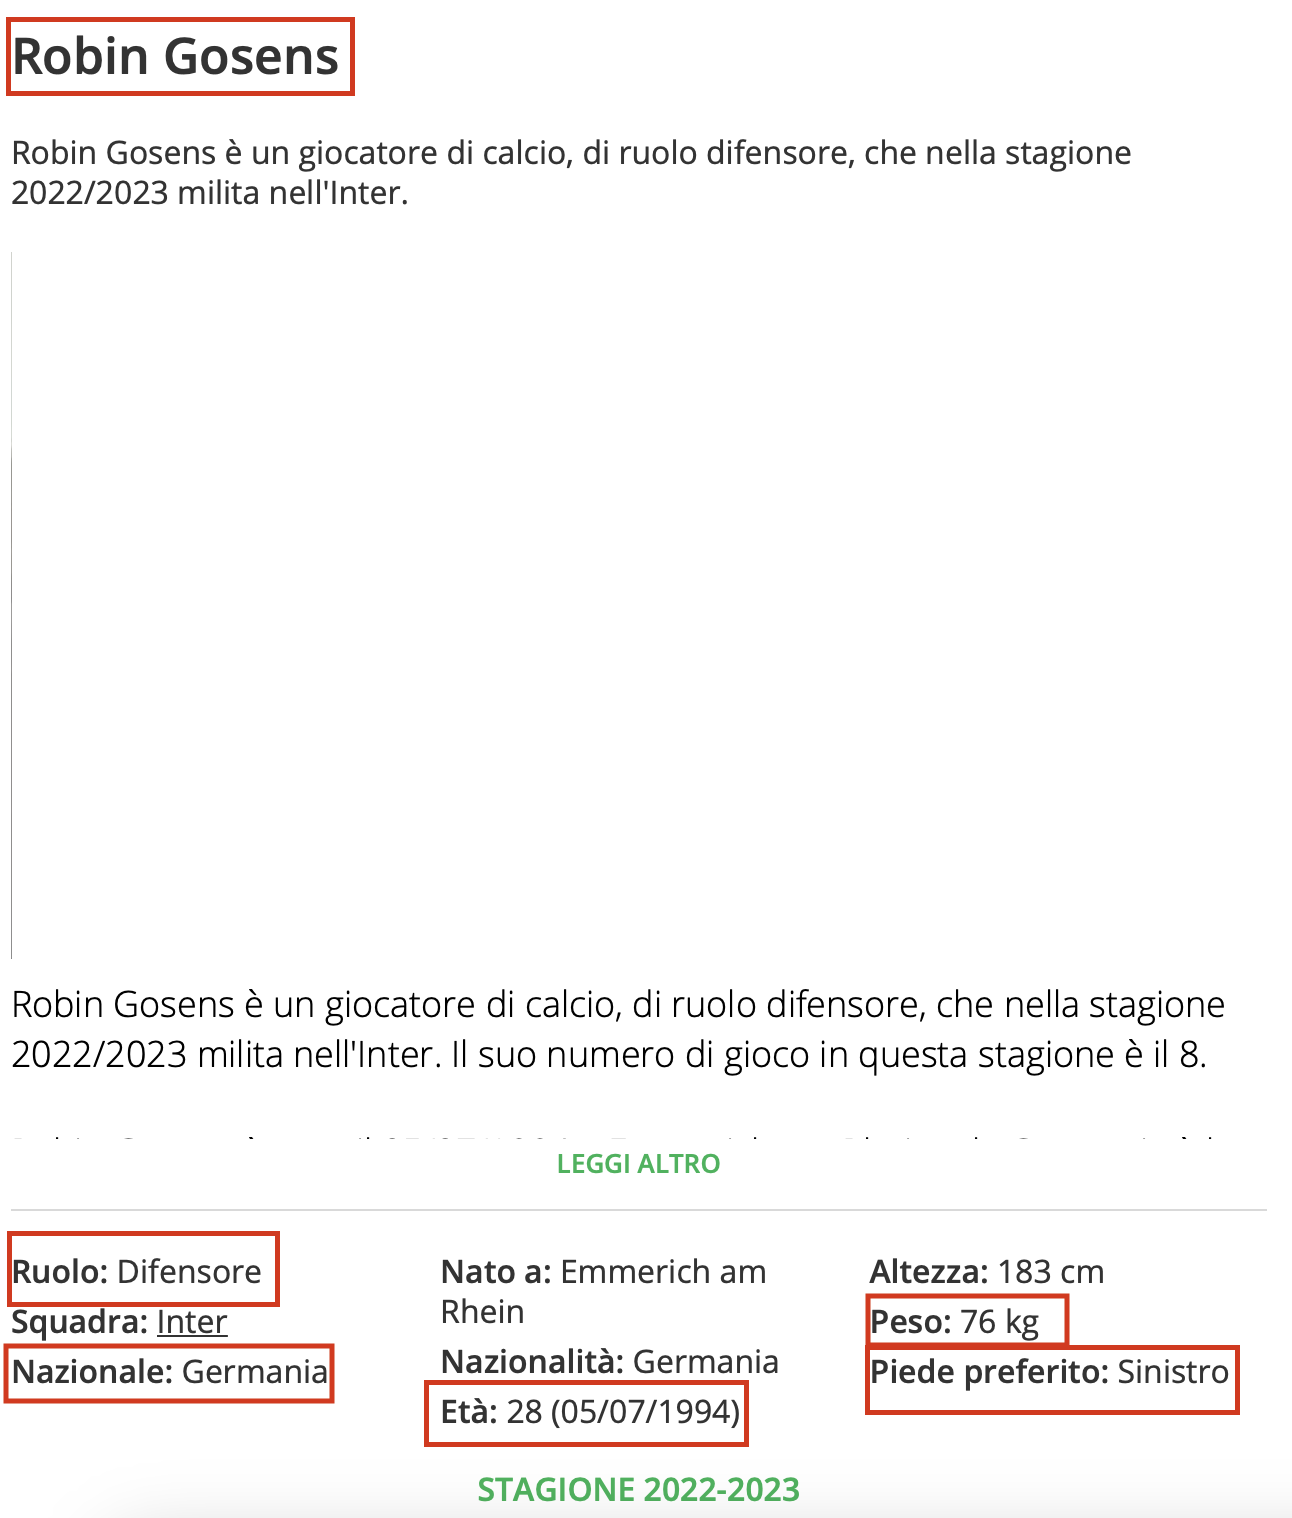
\includegraphics[scale=0.4]{img/virgilio1.png}
    \caption{Esempio pagina web Sport Virgilio}
    \label{fig:virgilio1}
\end{figure}
\begin{figure}
    \centering
    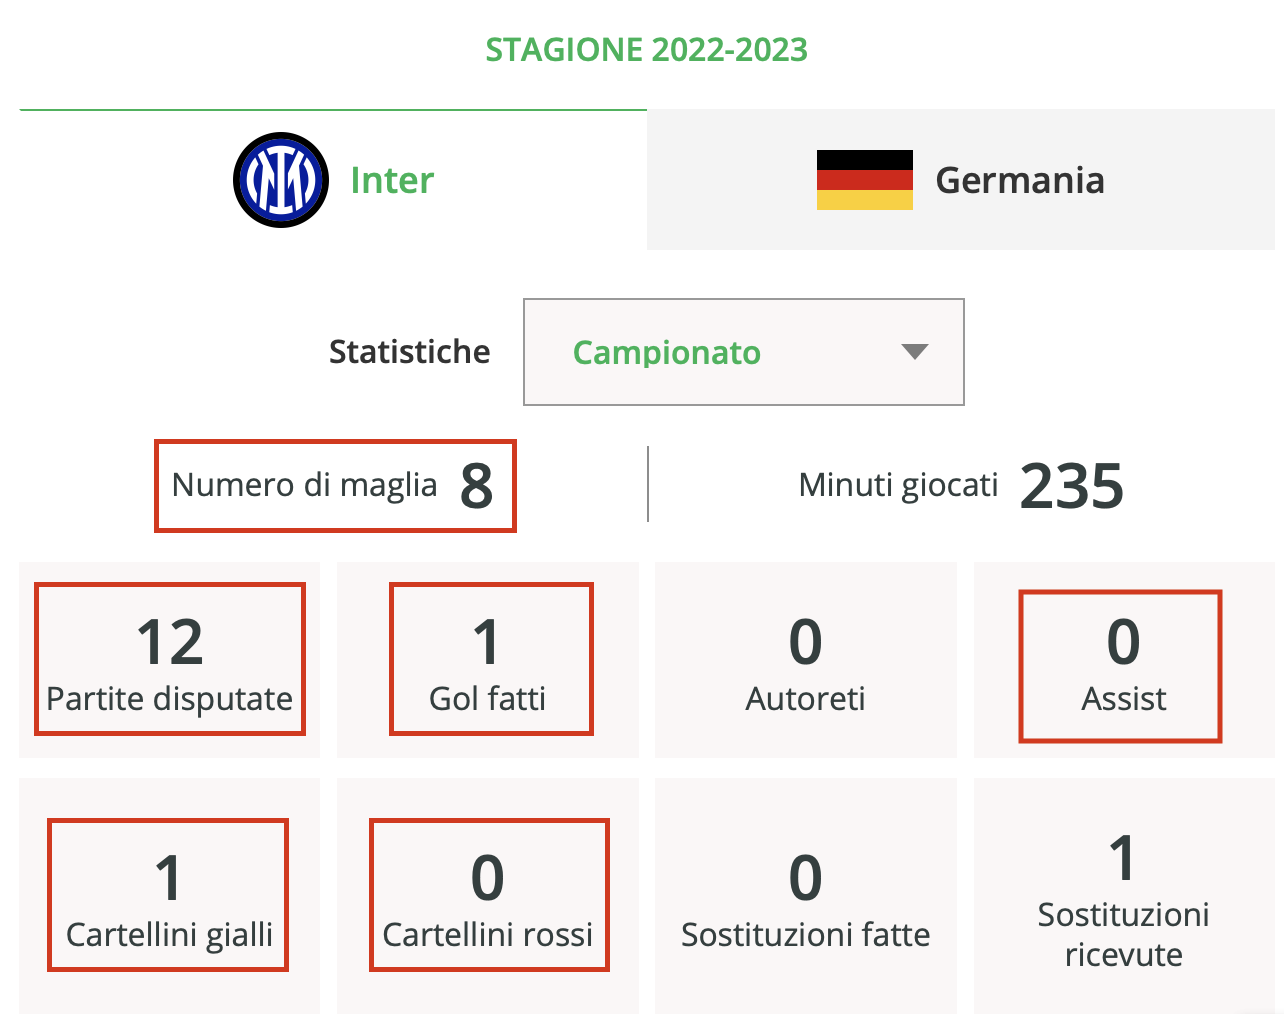
\includegraphics[scale=0.4]{img/virgilio2.png}
    \caption{Esempio pagina web Sport Virgilio (continuo di \ref{fig:virgilio1})}
    \label{fig:virgilio2}
\end{figure}

\subsection{Tuttocalciatori}
L'unico problema sollevato durante la verifica di efficacia delle espressioni usate per questo sito, è relativo all'estrazione del numero di gol. Poiché l'espressione usata riportava due valori, si è selezionato il primo di essi essendo coincidente con il dato richesto. 

Inoltre, nel sito non vengono mostrati gli assist.
\begin{table}[h!]
    \centering
    \begin{tabular}{|l|>{\color{xpath}}l|}
    \hline
        \textbf{Nome e Cognome} & \thead{\$x("//h1/text()")} \\
    \hline
        \textbf{Età} & \thead{\$x("//td[text()='Età']\\/following-sibling::td/text()")}\\
    \hline
        \textbf{Posizione} & \thead{\$x("(//strong[text()='RUOLO']\\/following-sibling::text())[1]")}\\
    \hline
        \textbf{Piede} & \thead{\$x("(//strong[text()='PIEDE CALCIO']\\/following-sibling::text())[1]")}\\
    \hline
        \textbf{Presenze} & \thead{\$x("(//*[contains(@class,'tr\_campionato')]\\/*[contains(text(),'2022-2023')]\\/following-sibling::td[3])[1]//text()")} \\
    \hline
        \textbf{Gol} & \thead{\$x("(//tr[contains(@class,'tr\_campionato')]\\/td[text()='2022-2023']\\/following-sibling::td[4]/strong/text())[1]")}\\
    \hline
        \textbf{Assist} & \thead{}\\
    \hline
        \textbf{Ammonizioni} & \thead{\$x("(//*[contains(@class,'tr\_campionato')]\\/*[contains(text(),'2022-2023')]\\/following-sibling::td[8])[1]//text()")}\\
    \hline
        \textbf{Espulsioni} & \thead{\$x("(//*[contains(@class,'tr\_campionato')]\\/*[contains(text(),'2022-2023')]\\/following-sibling::td[9])[1]//text()")}\\
    \hline
    \multicolumn{2}{|c|}{Caratteristiche aggiuntive} \\
    \hline
        \textbf{Scadenza contratto} & \thead{\$x("(//strong[text()='SCADENZA CONTRATTO']\\/following-sibling::text())[1]")}\\
    \hline
        \textbf{Procuratore} & \thead{\$x("(//strong[text()='PROCURATORE']\\/following-sibling::text())[1]")} \\
    \hline
        \textbf{Esordio in nazionale} & \thead{\$x("(//strong[text()='ESORDIO IN NAZIONALE']\\/following-sibling::text())[1]")} \\
    \hline
    %     \textbf{Presenze in nazionale} & \thead{\$x("(//strong[text()='PRESENZE IN NAZIONALE']\\/following-sibling::text())[1]")} \\
    % \hline
    %     \textbf{Presenze nei campionati} & \thead{\$x("//tr[contains(@class,'tr\_campionato totale')]\\/td[4]/text()")} \\
    % \hline
    \end{tabular}
    \caption{Caratteristiche ed espressioni per Tuttocalciatori}
    \label{tab:my_label}
\end{table}
\begin{figure}
    \centering
    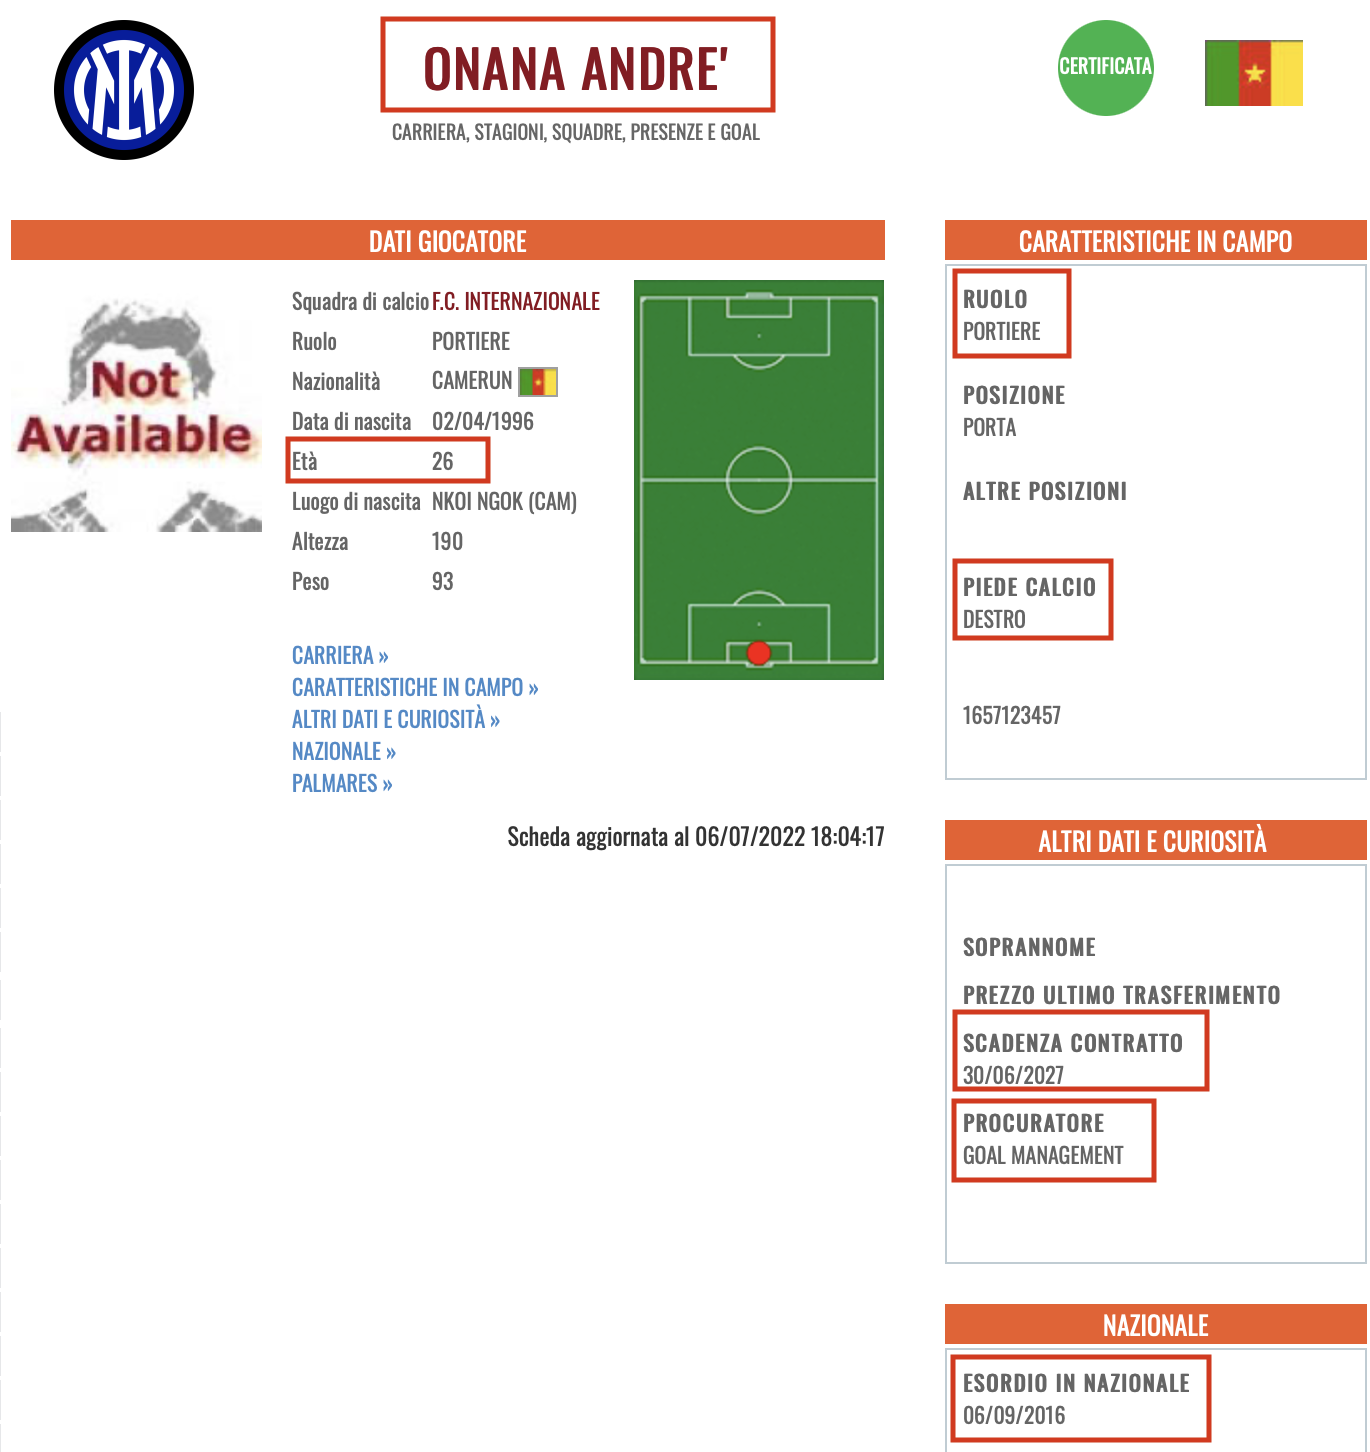
\includegraphics[scale=0.4]{img/tuttocalc1.png}
    \caption{Esempio pagina web Tuttocalciatori}
    \label{fig:tuttocalc1}
\end{figure}
\begin{figure}
    \centering
    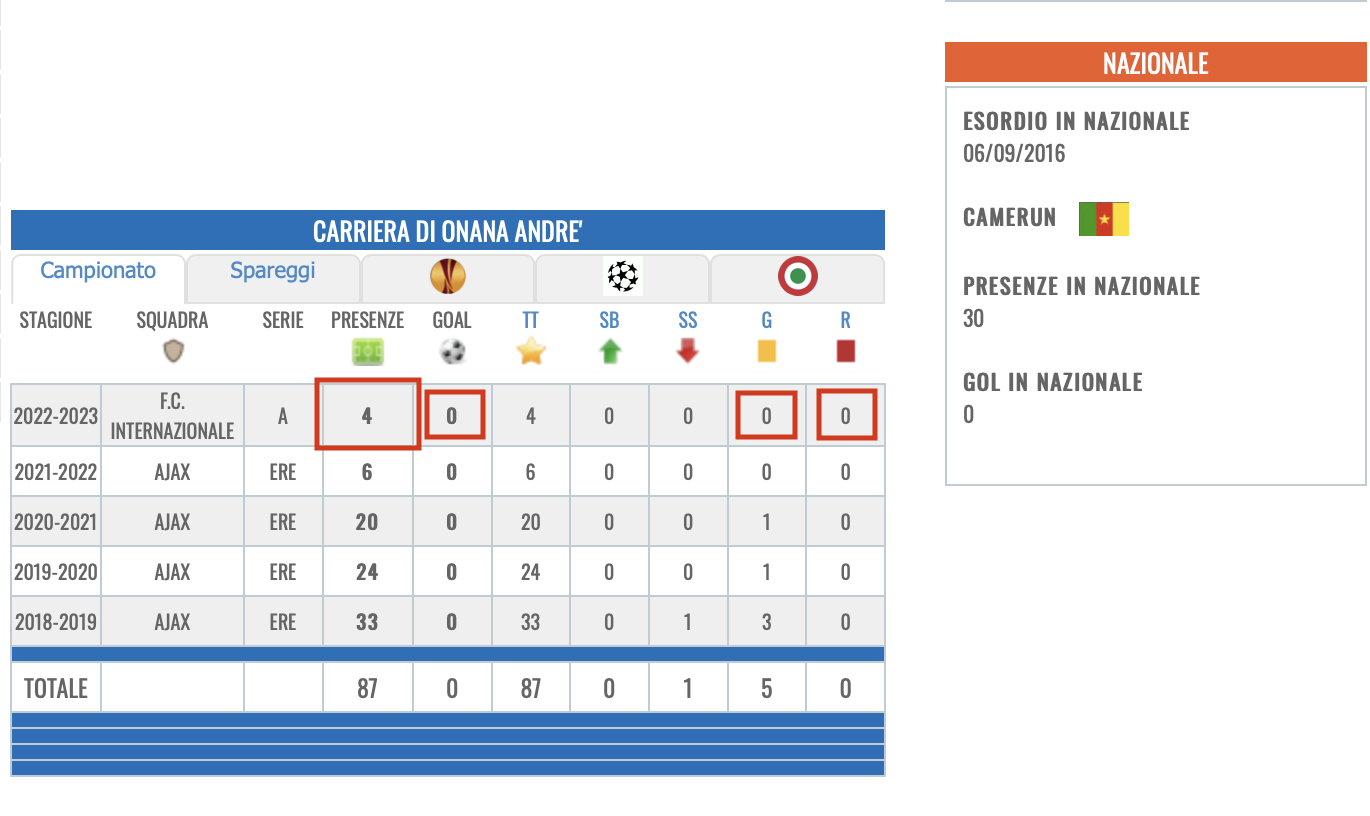
\includegraphics[scale=0.4]{img/tuttocalc2.png}
    \caption{Esempio pagina web Tuttocalciatori (continuo \ref{fig:tuttocalc1}}
    \label{fig:tuttocalc2}
\end{figure}

\subsection{Football Database}\label{se:fdb}
Il maggior numero di problemi sono stati riscontrati in questo sito, in cui le informazioni e statistiche dei giocatori venivano posizionate diversamente in base al ruolo del giocatore. Di conseguenza, per verificare l'efficacia complessiva delle espressioni usate, sono state selezionate pagine web relative a calciatori di tutti i ruoli. 

Per quanto riguarda questa caratteristica, inoltre, si è deciso di elencare tutte le posizioni che il sito proponeva circa un giocatore, al posto di ritornare la posizione che ricopre più di frequente, questo ha richiesto l'utilizzo della clausola \texttt{or}.
\begin{table}[h!]
    \centering
    \begin{tabular}{|l|>{\color{xpath}}l|}
    \hline
        \textbf{Nome e Cognome} & \thead{\$x("//h1/span[contains(@class,'lastname')]\\/..//text()")} \\
    \hline
        \textbf{Età} & \thead{\$x("//*[@class='age']/text()")}\\
    \hline
        \textbf{Posizione} & \thead{\$x("//tr[contains(@class,'mainposition') or\\ contains(@class,'otherposition')]/td[1]/text()")}\\
    \hline
        \textbf{Piede} & \thead{\$x("//span[contains(text(),'Best foot')]\\/following-sibling::text()")}\\
    \hline
        \textbf{Presenze} & \thead{\$x("//*[contains(text(),'Played matches')]\\/preceding-sibling::*/text()")} \\
    \hline
        \textbf{Gol} & \thead{\$x("//span[text()='Goals']\\/preceding-sibling::span[1]/text()")}\\
    \hline
        \textbf{Assist} & \thead{\$x("//*[contains(text(),'Assists')]\\/preceding-sibling::*[1]/text()")}\\
    \hline
        \textbf{Ammonizioni} & \thead{\$x("//span[text()='Yellow cards']\\/preceding-sibling::span[1]/text()")}\\
    \hline
        \textbf{Espulsioni} & \thead{\$x("//span[text()='Red cards']\\/preceding-sibling::span[1]/text()")}\\
    \hline
    \multicolumn{2}{|c|}{Caratteristiche aggiuntive} \\
    \hline
        \textbf{Squadra} & \thead{\$x("//div[contains(@class,'clublogo')]/a/text()")}\\
    \hline
        \textbf{Minuti giocati} & \thead{\$x("//span[text()='Minutes played']\\/preceding-sibling::span[1]/text()")}\\
    \hline
    %     \textbf{Peso} & \thead{\$x("//span[contains(text(),'Weight')]\\/following-sibling::text()")}\\
    % \hline
    \end{tabular}
    \caption{Caratteristiche ed espressioni per Football Database}
    \label{tab:my_label}
\end{table}
\begin{figure}
    \centering
    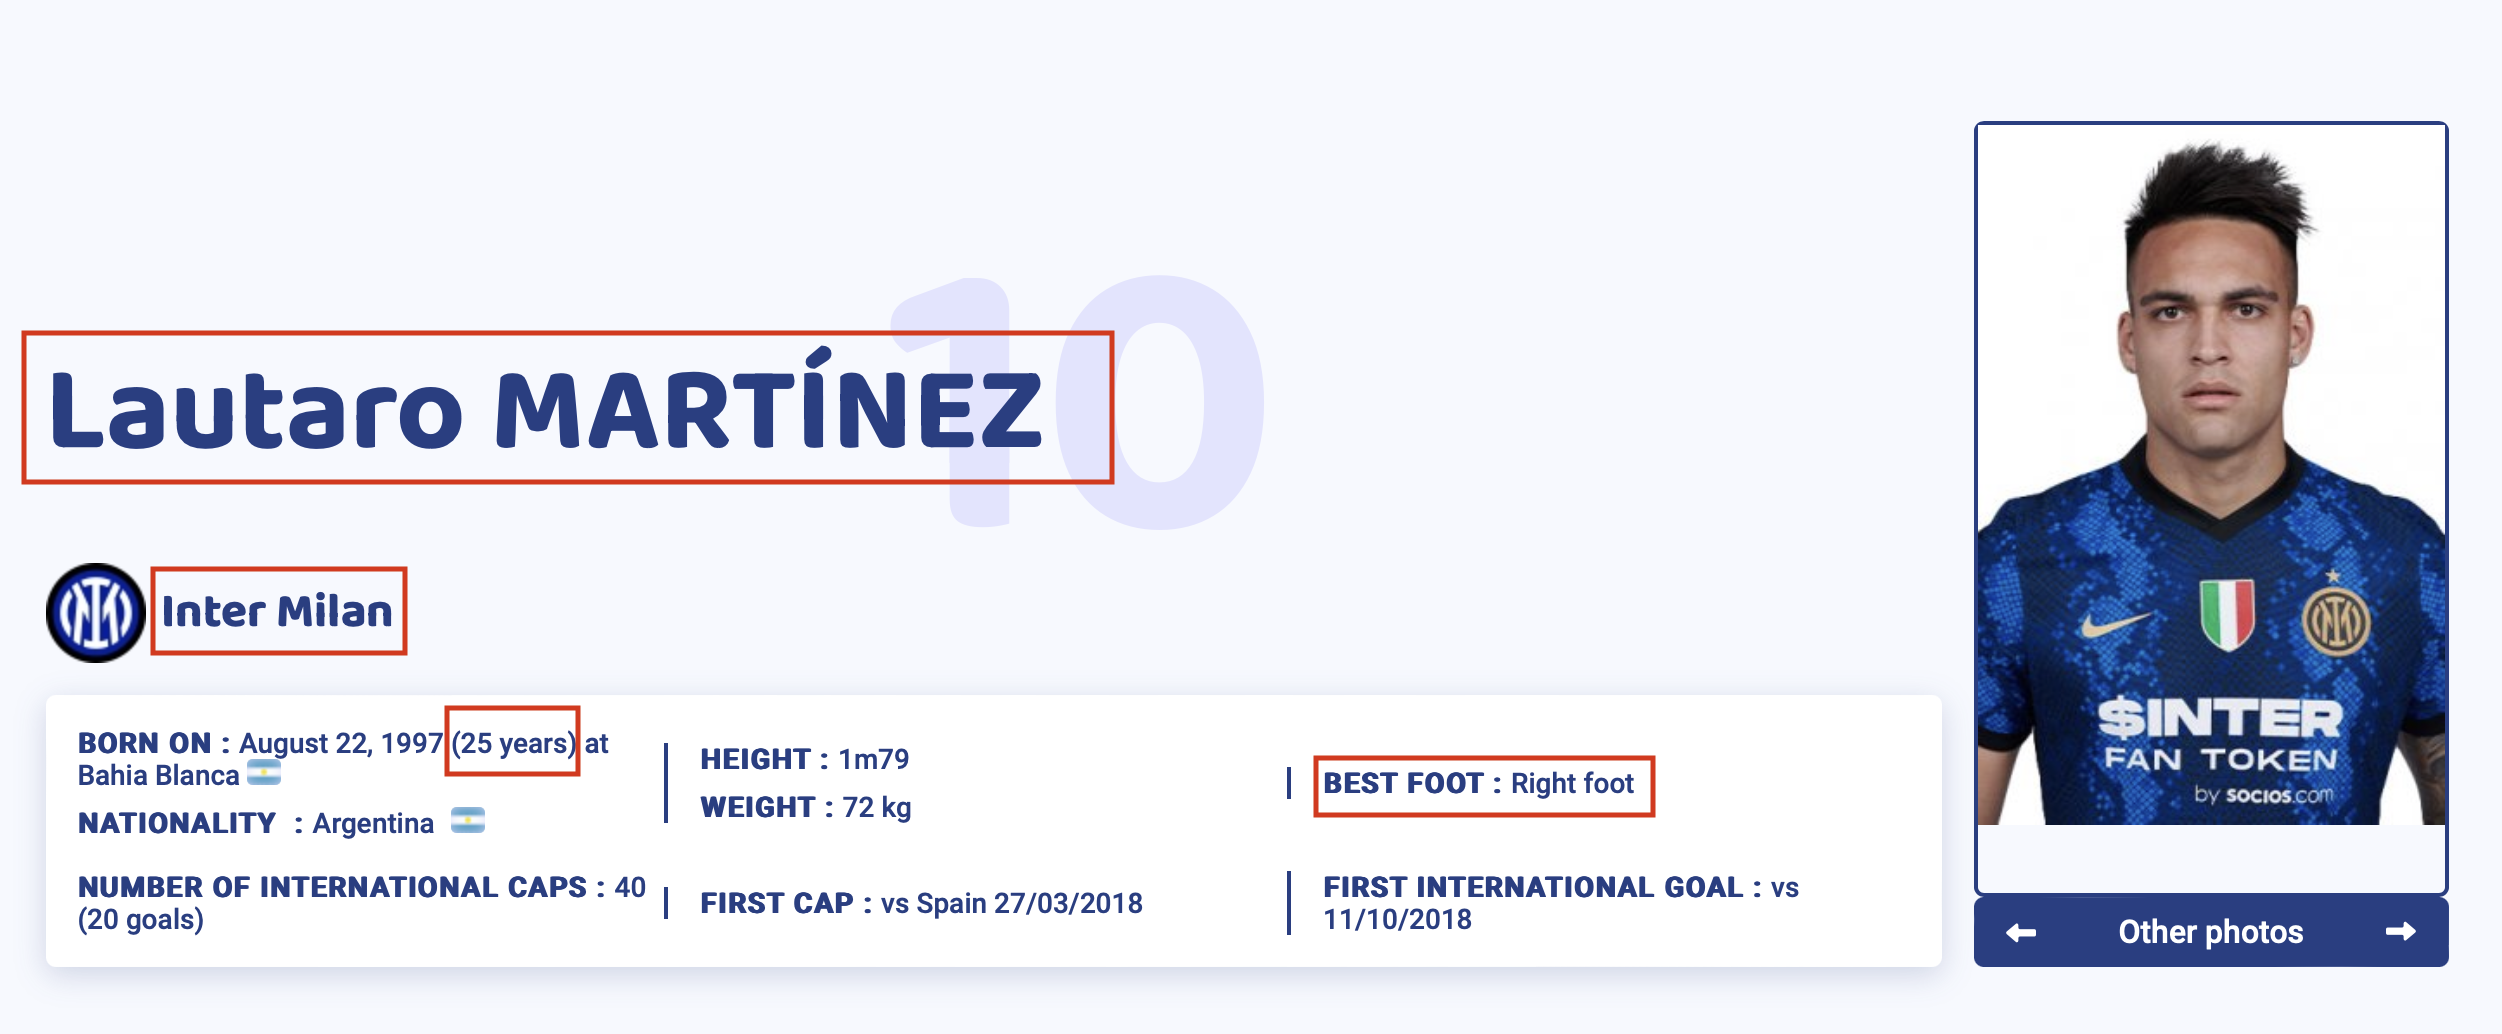
\includegraphics[scale=0.3]{img/footdb1.png}
    \caption{Esempio pagina web Football database (1)}
    \label{fig:footdb1}
\end{figure}
\begin{figure}
    \centering
    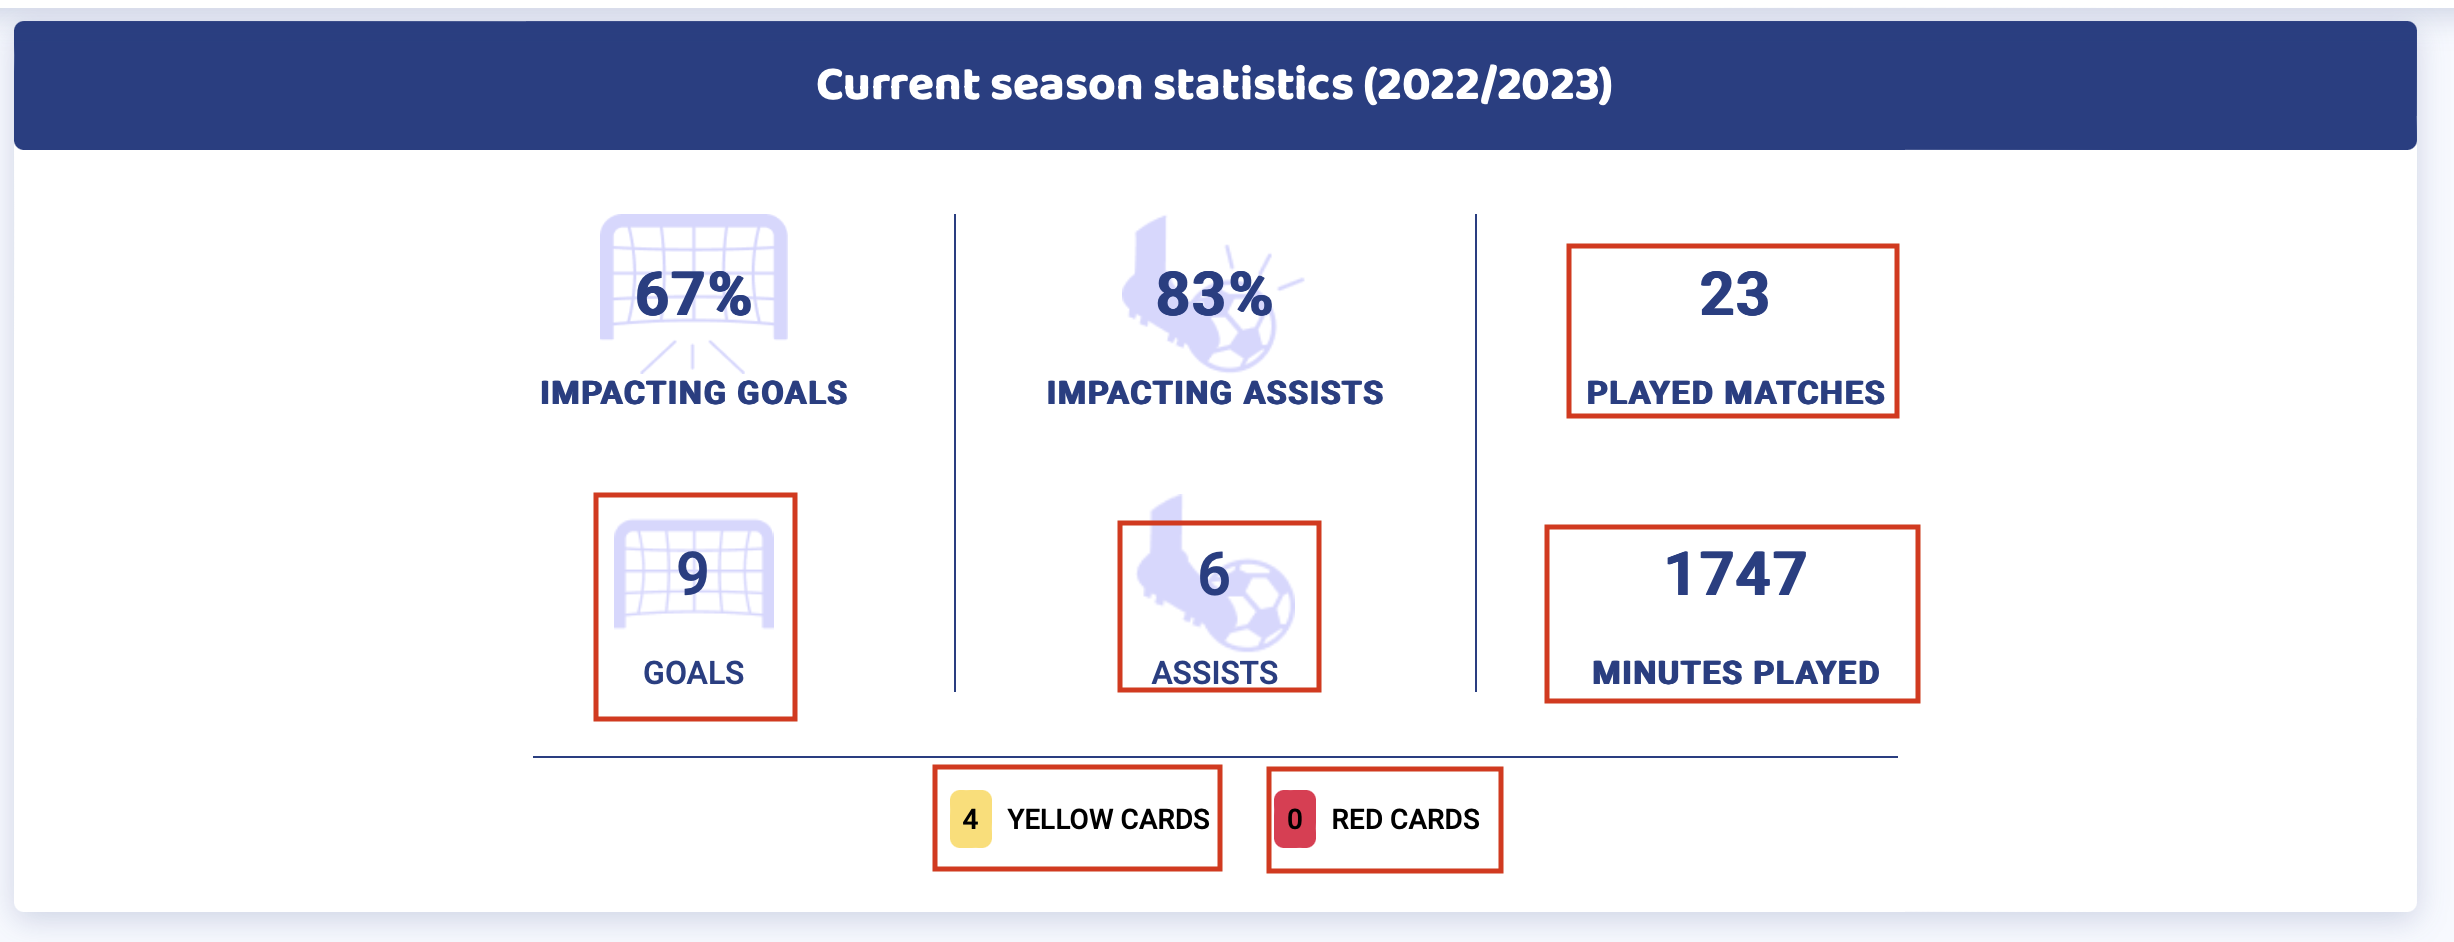
\includegraphics[scale=0.3]{img/footdb2.png}
    \caption{Esempio pagina web Football database (2)}
    \label{fig:footdb2}
\end{figure}
\begin{figure}
    \centering
    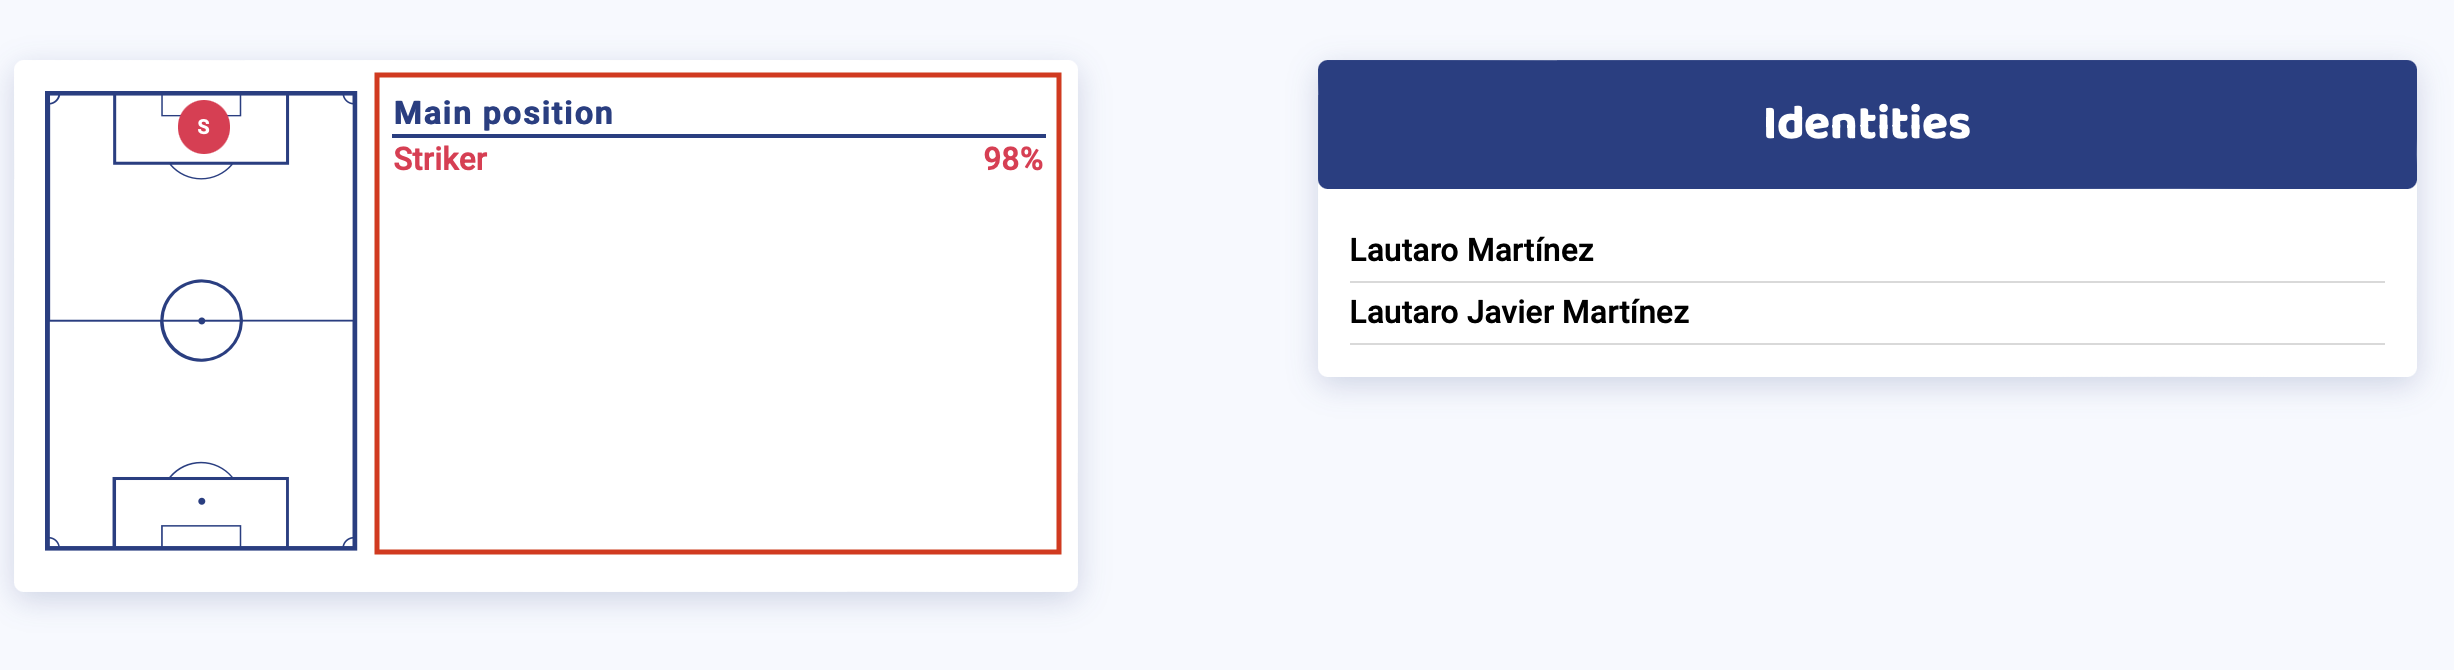
\includegraphics[scale=0.3]{img/footdb3.png}
    \caption{Esempio pagina web Football database (3)}
    \label{fig:footdb3}
\end{figure}